%% Full length research paper template
%% Created by Simon Hengchen and Nilo Pedrazzini for the Journal of Open Humanities Data (https://openhumanitiesdata.metajnl.com)

\documentclass{article}
\usepackage[english]{babel}
\usepackage[utf8]{inputenc}
\usepackage{johd}
\usepackage{indentfirst}

\title{Interaction of Charged Particles with Different Materials}

\author{Sharod Roy\\
        \small Institute for Computing in Research, Santa Fe, NM \\
        \small Leon M. Goldstein High School for the Sciences, Brooklyn, NY \\
        \small Email: \tt{sharodroy7@gmail.com} \\
}

\date{} %leave blank

\begin{document}

\maketitle

\begin{abstract} 
This paper evaluates the interactions of charged particles with various materials using the Geant4 simulation software developed by CERN. Geant4 employs Monte Carlo methods to simulate particle interactions within a detector plane, enabling visualization and analysis of particle scattering behaviors. The study investigates three main parameters: slab material, particle type, and energy level. The materials examined are Aluminum (Al), Gold (Au), Iron (Fe), Plastic, and Uranium (U), chosen for their varying atomic properties. Charged particles analyzed include protons, electrons, positively charged muons, and negatively charged muons, representing a diverse set of interactions. The energy levels tested are 100 MeV, 10,000 MeV, and 100,000 MeV, covering a broad range of kinetic energies. Results indicate significant variations in scattering patterns and momentum distributions across different materials and energies, providing insights into the underlying physical processes. These findings contribute to a deeper understanding of particle-material interactions, with potential applications in nuclear physics, material science, and radiation shielding.
\end{abstract}

\section{Introduction}

The interaction of charged particles with matter is a fundamental topic in physics, with broad implications across various fields, including nuclear physics, material science, medical imaging, and radiation therapy. Understanding how particles such as protons, electrons, and muons interact with different materials at varying energy levels provides crucial insights into the underlying principles of particle physics and aids in the development of new technologies and applications. This study aims to explore these interactions using Geant4, a simulation toolkit developed by CERN.

Geant4 is a powerful tool for modeling the passage of particles through matter. It employs Monte Carlo methods to simulate complex physical processes, making it an essential resource for researchers in high-energy physics, space science, and medical physics. By utilizing Geant4, scientists can create detailed simulations of particle interactions, enabling precise predictions of behavior in real-world scenarios.

In this study, we investigate the interactions of protons, electrons, and muons with five different materials: Aluminum (Al), Gold (Au), Iron (Fe), Plastic, and Uranium (U). These materials were chosen for their diverse atomic properties and practical significance in various applications. For instance, aluminum is widely used in aerospace engineering due to its lightweight and corrosion-resistant properties, while uranium is critical in nuclear reactors and weapons.

The energy levels considered in this study range from 1,000 MeV to 100,000 MeV, covering a broad spectrum of particle velocities and interaction intensities. This range allows for a comprehensive examination of how energy influences the scattering, absorption, and transmission of particles through different materials.

\noindent\textbf{The primary objectives of this research are to:}

Analyze the scattering patterns of charged particles as they pass through different materials.
Investigate how the type of material and energy level affect particle behavior.
Provide insights into the momentum distribution and energy deposition patterns of particles in these materials.
By achieving these objectives, the study seeks to contribute valuable data and insights that can enhance the understanding of particle-material interactions. These findings may have implications for improving radiation shielding, optimizing detector design, and advancing various scientific and industrial applications.

\section{Background}

The study of charged particle interactions with matter is a cornerstone of modern physics, tracing its origins back to early 20th-century experiments that unveiled the atomic structure of matter. As researchers have delved deeper into the quantum world, understanding how particles such as protons, electrons, and muons interact with different materials has become increasingly important. This knowledge forms the basis for various applications, from fundamental research in particle physics to practical implementations in medical diagnostics and treatment.

\subsection{Historical Context}

The investigation of particle interactions began with pioneering experiments by Ernest Rutherford, who used alpha particles to probe the atomic nucleus, leading to the discovery of the proton. Since then, the study of particle interactions has evolved significantly, driven by advancements in experimental techniques and theoretical models. The development of particle accelerators and detectors has enabled scientists to explore particle behavior at unprecedented energy levels, revealing the intricacies of particle interactions with matter.

\subsection{Modern Applications}

In the field of medical physics, charged particles are utilized in imaging techniques such as Positron Emission Tomography (PET) and radiation therapies like Proton Beam Therapy. These applications rely on the precise understanding of particle interactions to optimize the accuracy and efficacy of treatments. Similarly, in material science, the analysis of particle interactions aids in the development of radiation-resistant materials and the improvement of nuclear reactor safety.

\subsection{Theoretical Foundations}

Theoretical models describing particle interactions with matter are grounded in quantum mechanics and electrodynamics. The Bethe-Bloch equation, for example, quantifies the energy loss of charged particles as they traverse a medium, providing insights into their stopping power and range. Additionally, Monte Carlo simulations have become a standard tool for modeling complex particle interactions, offering detailed predictions of scattering patterns and energy deposition.

\subsection{Geant4 Simulation Toolkit}

Geant4, a widely used simulation toolkit developed by CERN, has revolutionized the study of particle interactions. Its ability to model the passage of particles through matter using Monte Carlo methods has made it an indispensable resource for researchers across various disciplines. Geant4's versatility allows for the simulation of diverse physical processes, from electromagnetic interactions to hadronic processes, facilitating comprehensive analyses of particle behavior.

\subsection{Research Gaps and Motivation}

Despite significant advancements, several challenges remain in the field of particle-material interactions. Existing studies often focus on specific materials or energy levels, leaving gaps in our understanding of how different parameters influence particle behavior. Additionally, the need for more detailed simulations and data analysis persists, especially in emerging fields like nanotechnology and space exploration.

This study aims to address these gaps by systematically investigating the interactions of protons, electrons, and muons with a range of materials at varying energy levels. By employing Geant4 simulations, this research seeks to provide valuable data and insights that can enhance our understanding of particle-material interactions and inform future scientific and industrial applications.

\section{Methods}

\subsection{Geant4 Simulation Setup}

The Geant4 simulation toolkit was used to model the interactions of charged particles with matter. Geant4 is a robust platform that utilizes Monte Carlo methods to simulate the passage of particles through complex geometries, enabling precise predictions of scattering patterns, energy deposition, and particle trajectories.

\begin{itemize}
    \item \textbf{Simulation Environment:} The simulation environment was constructed to mimic a typical experimental setup, with particles directed towards a slab of the target material. The geometry was defined to include a source of particles, the target material slab, and a detector plane positioned behind the target to capture scattered particles.

    \item \textbf{Geometry Definition:} A cubic world volume was defined, within which a slab of the target material was placed. The slab thickness was chosen to ensure significant interaction without complete attenuation of the incident particles.

    \item \textbf{Physics Processes:} The simulation incorporated relevant electromagnetic and hadronic processes, allowing for accurate modeling of particle interactions. Geant4's built-in physics lists were utilized to account for processes such as ionization, bremsstrahlung, multiple scattering, and nuclear interactions.
\end{itemize}

\begin{figure}[H]
\centering
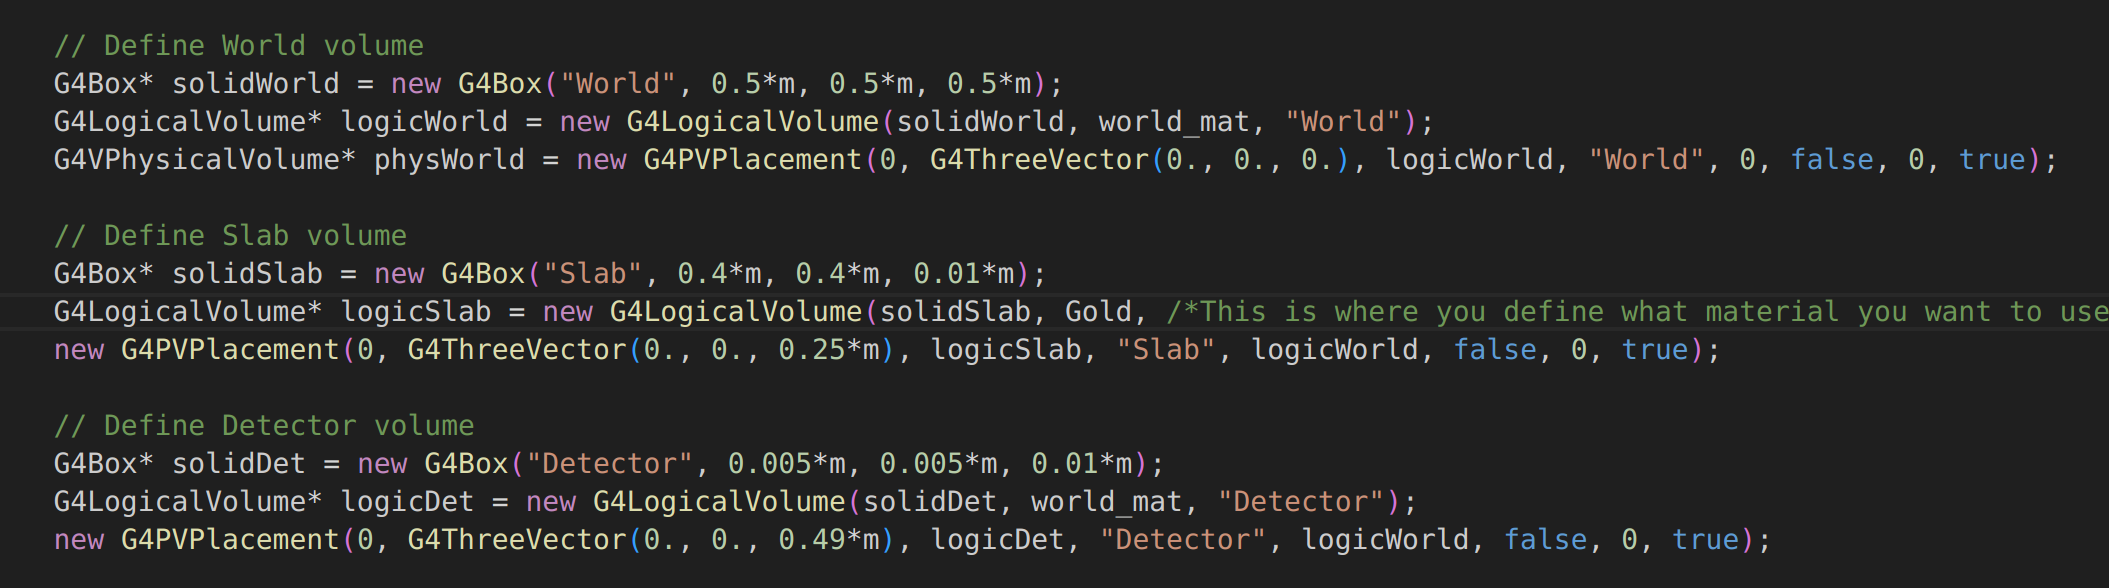
\includegraphics[width=1\textwidth]{Screenshot from 2024-07-31 20-31-58.png}
\caption{Geometry of Simulation}
\end{figure}

\begin{figure}[H]
\centering
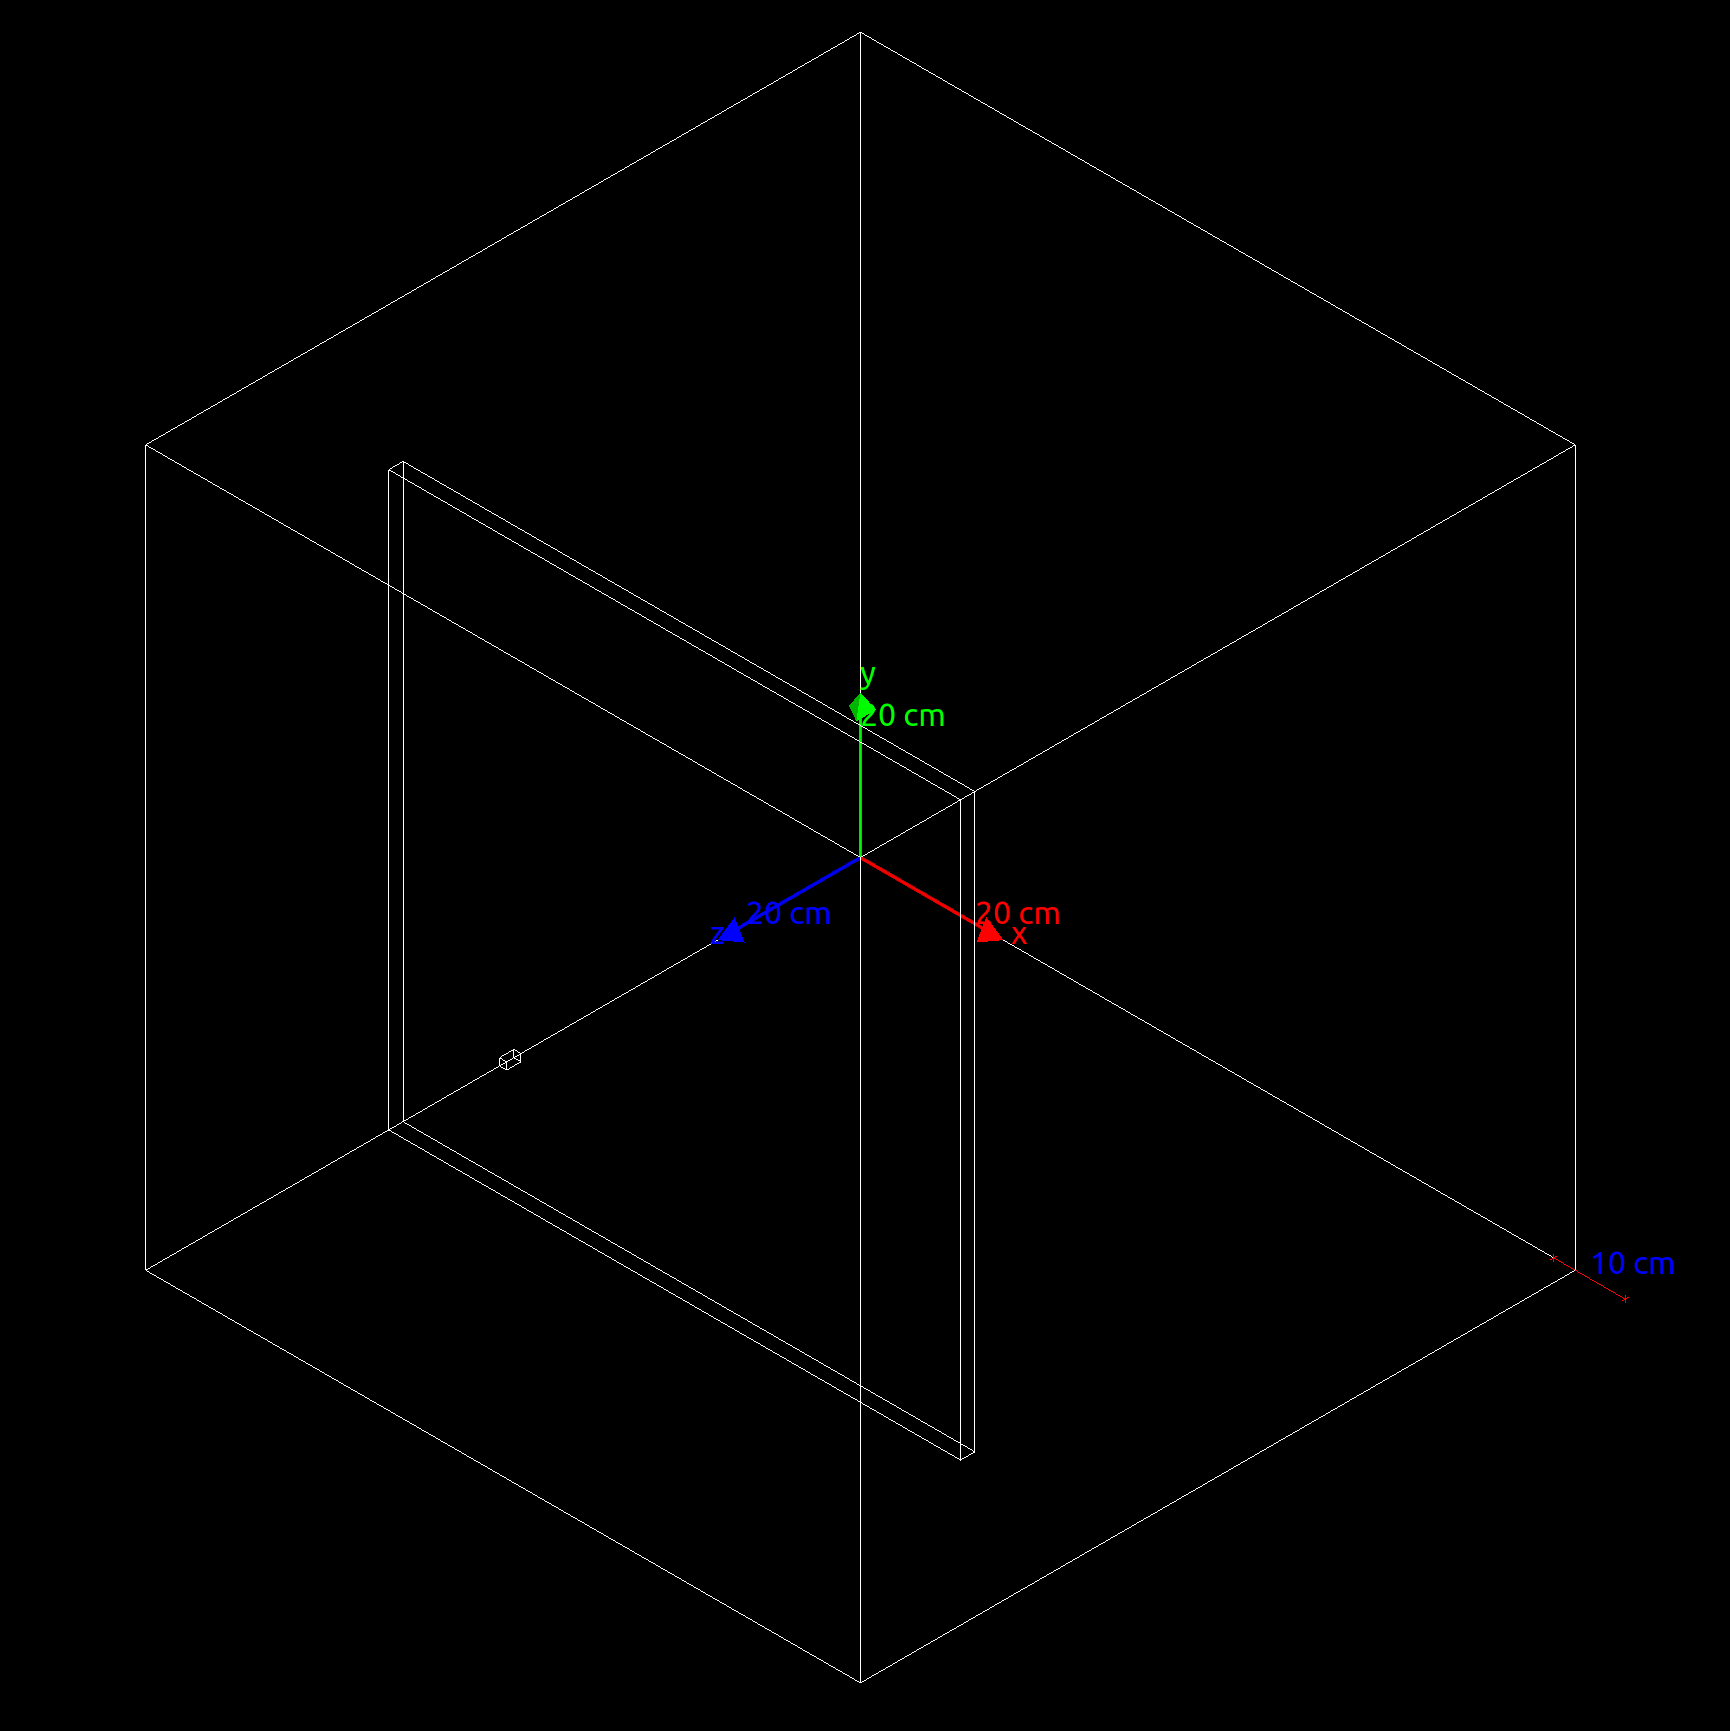
\includegraphics[width=0.65\textwidth]{Screenshot from 2024-07-31 20-26-55.png}
\caption{Visualization of Geometry}
\end{figure}

\subsection{Materials and Particle Parameters}

\begin{itemize}
    \item \textbf{Materials:} The study focused on five materials: Aluminum (Al), Gold (Au), Iron (Fe), Plastic, and Uranium (U). The materials were selected for their varying atomic numbers, densities, and practical applications. Material properties, such as density and atomic composition, were defined according to standard Geant4 material libraries.

    \item \textbf{Particle Types:} The particles investigated included protons, electrons, positively charged muons, and negatively charged muons. These particles were chosen due to their relevance in various scientific and industrial applications.

    \item \textbf{Energy Levels:} Three distinct energy levels were selected for the study: 100 MeV, 10,000 MeV, and 100,000 MeV. This range encompasses typical energies encountered in particle accelerators and radiation therapy applications, allowing for a comprehensive analysis of energy-dependent interactions.
\end{itemize}

\begin{figure}[H]
\centering
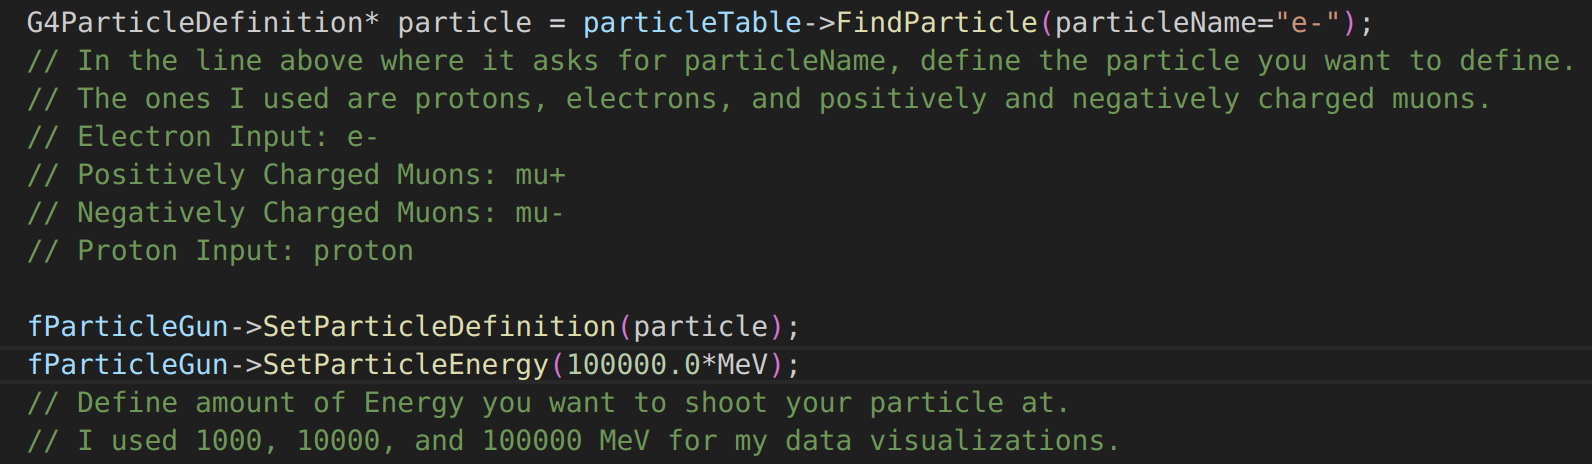
\includegraphics[width=0.65\textwidth]{Screenshot from 2024-07-31 20-43-33.png}
\caption{Implementation of Particle Gun}
\end{figure}

\subsection{Simulation Procedure}

\begin{enumerate}
    \item \textbf{Initialization:} The simulation was initialized with the chosen particle type, energy level, and material. A primary generator was used to emit particles towards the target slab.

    \item \textbf{Particle Tracking:} Geant4 tracked the particles as they interacted with the material, recording data on scattering angles, energy loss, and secondary particle production.

    \item \textbf{Data Collection:} A detector plane positioned behind the target slab collected data on transmitted and scattered particles. Parameters such as position, momentum, and energy were recorded for further analysis.

    \item \textbf{Repetition:} The simulation was repeated for each combination of particle type, material, and energy level, ensuring comprehensive coverage of the parameter space.
\end{enumerate}

\begin{figure}[H]
\centering
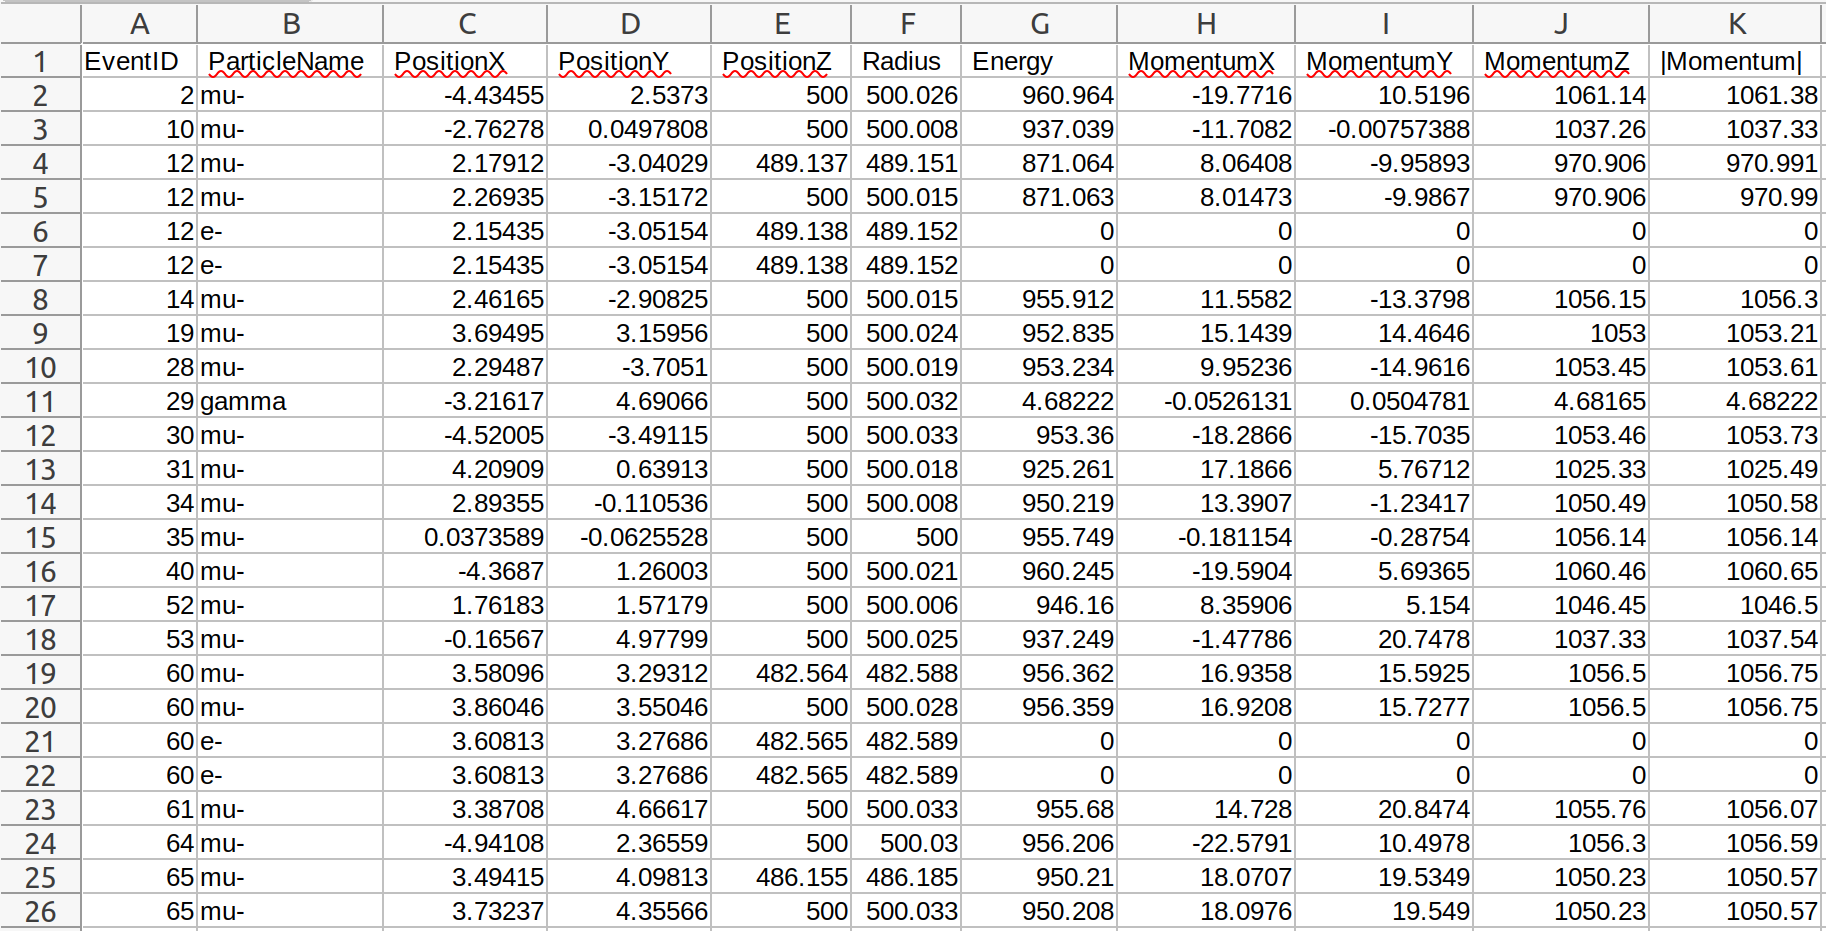
\includegraphics[width=0.9\textwidth]{Screenshot from 2024-08-02 13-05-09.png}
\caption{Example Data Collection in .csv file}
\end{figure}

\subsection{Graphical Data Representation}
\begin{itemize}
    \item \textbf{Position X vs. Position Y:} This scatter plot graph illustrates the spatial distribution of particles on the detector plane. By plotting the Position X (horizontal position) against Position Y (vertical position), you can visualize the scattering patterns of particles after they interact with the material. This graph reveals how particles spread across the detector plane, identifying regions of high or low particle density and possible symmetrical or asymmetrical patterns. The analysis of this graph can highlight the uniformity or concentration of particle impacts, which may indicate the nature of interactions such as scattering angles or potential energy barriers within the material. It is particularly useful for understanding scattering behavior and verifying theoretical predictions about particle dispersion.

    \item \textbf{Number of Particles vs. Radius of Detector Plane:} 

\textit{Formula for Radius of Detector Plane (Magnitude of Position):}
\[
|\mathbf{r}| = \sqrt{x^2 + y^2 + z^2}
\]

    
    This histogram plots the Number of Particles detected against the Radius of the Detector Plane. By examining how the number of particles varies with distance from the center, this graph assesses the distribution of particle interactions across different radial positions. It measures the radial distribution of particles and understands how many particles reach specific areas of the detector. Peaks or troughs in this graph can indicate preferred scattering angles, absorption by the material, or the presence of resonances. This information is vital for designing detector systems and understanding how the spatial configuration affects particle detection efficiency.

    \item \textbf{Momentum vs. Frequency of Momentum:} 

\textit{Formula for Magnitude of Momentum:}
\[
|\mathbf{p}| = \sqrt{p_x^2 + p_y^2 + p_z^2}
\]
    
    This histogram displays \textbf{Momentum} (p) on the x-axis against the \textbf{Frequency of Momentum} occurrences on the y-axis. It provides insights into the momentum distribution of particles before and after interactions with the material. By observing changes in momentum distribution, this graph provides clues about the energy transfer and interaction dynamics between particles and material. Shifts in momentum can indicate energy loss or gain, and peaks in the distribution can show the most probable momentum values. This analysis is crucial for understanding how particles transfer energy within materials and for validating conservation of momentum principles in different interaction scenarios.

\end{itemize}

\subsection{Software and Hardware Specifications}

\begin{itemize}
    \item \textbf{Software:} The simulations were conducted using Geant4 version 10.7.2. The data analysis was performed using Python with libraries such as Matplotlib and Pandas for data handling and visualization.

    \item \textbf{Hardware:} The simulations were run on a Dell XPS 2-in-1 9315 computer, ensuring sufficient computational resources for the Monte Carlo simulations.
\end{itemize}

\section{Results and discussion}

\subsection{Position X vs. Position Y}

\subsubsection{Protons}

\begin{figure}[H]
\centering
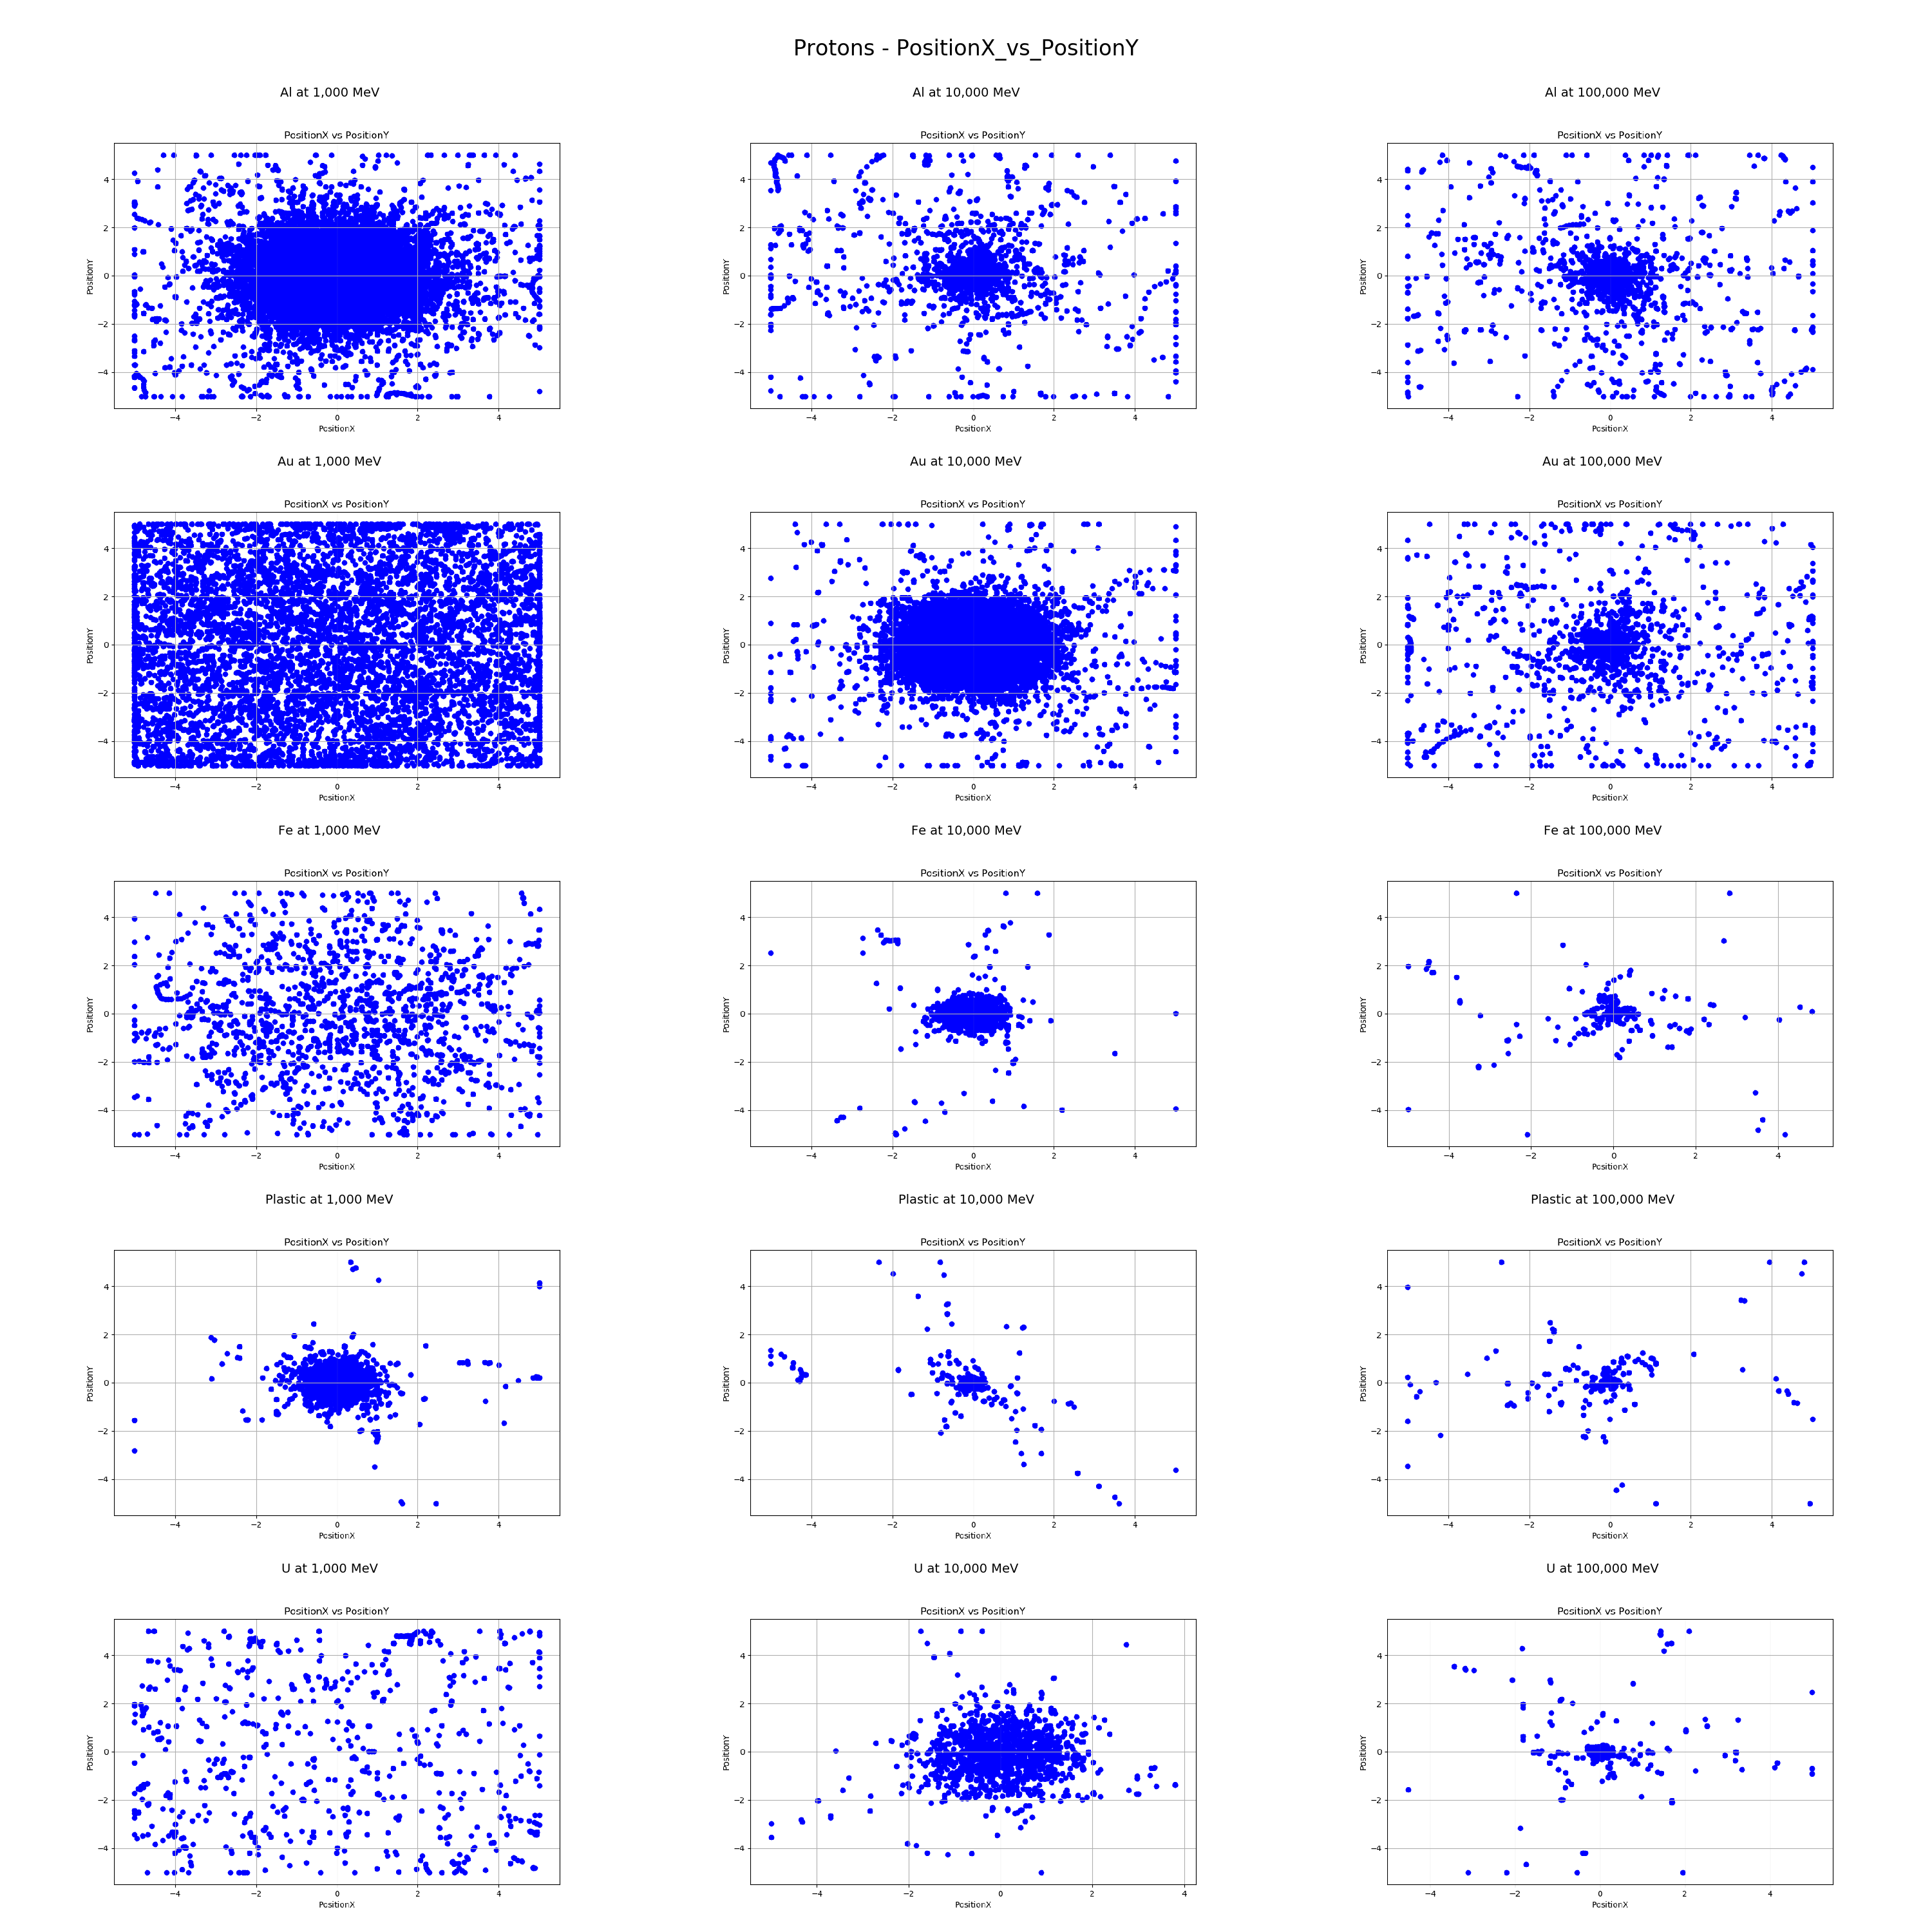
\includegraphics[width=0.9\textwidth]{images/Combined Plots/PositionX_vs_PositionY_p.png}
\end{figure}\

\noindent At 1,000 MeV, Aluminum shows a spread with most impacts within ±2 units on both axes, expanding to ±5 units at 100,000 MeV, indicating increased scattering with higher energy. Gold has a tight cluster within ±1 unit at 1,000 MeV due to its high stopping power, spreading to ±4 units at 100,000 MeV. Iron exhibits a uniform distribution, with impacts within ±3 units at 1,000 MeV and extending to ±5 units at 100,000 MeV. Plastic shows the broadest spread, from ±3 units at 1,000 MeV to ±5 units at 100,000 MeV, indicating less resistance to proton penetration. Uranium, similar to Gold, shows a tight cluster within ±1 unit at 1,000 MeV, spreading to ±4 units at 100,000 MeV. These results indicate that higher proton energies lead to increased scattering across all materials, with heavier materials like Gold and Uranium showing denser central clusters, reflecting their higher stopping power compared to lighter materials like Plastic.

\subsubsection{Electrons}

\begin{figure}[H]
\centering
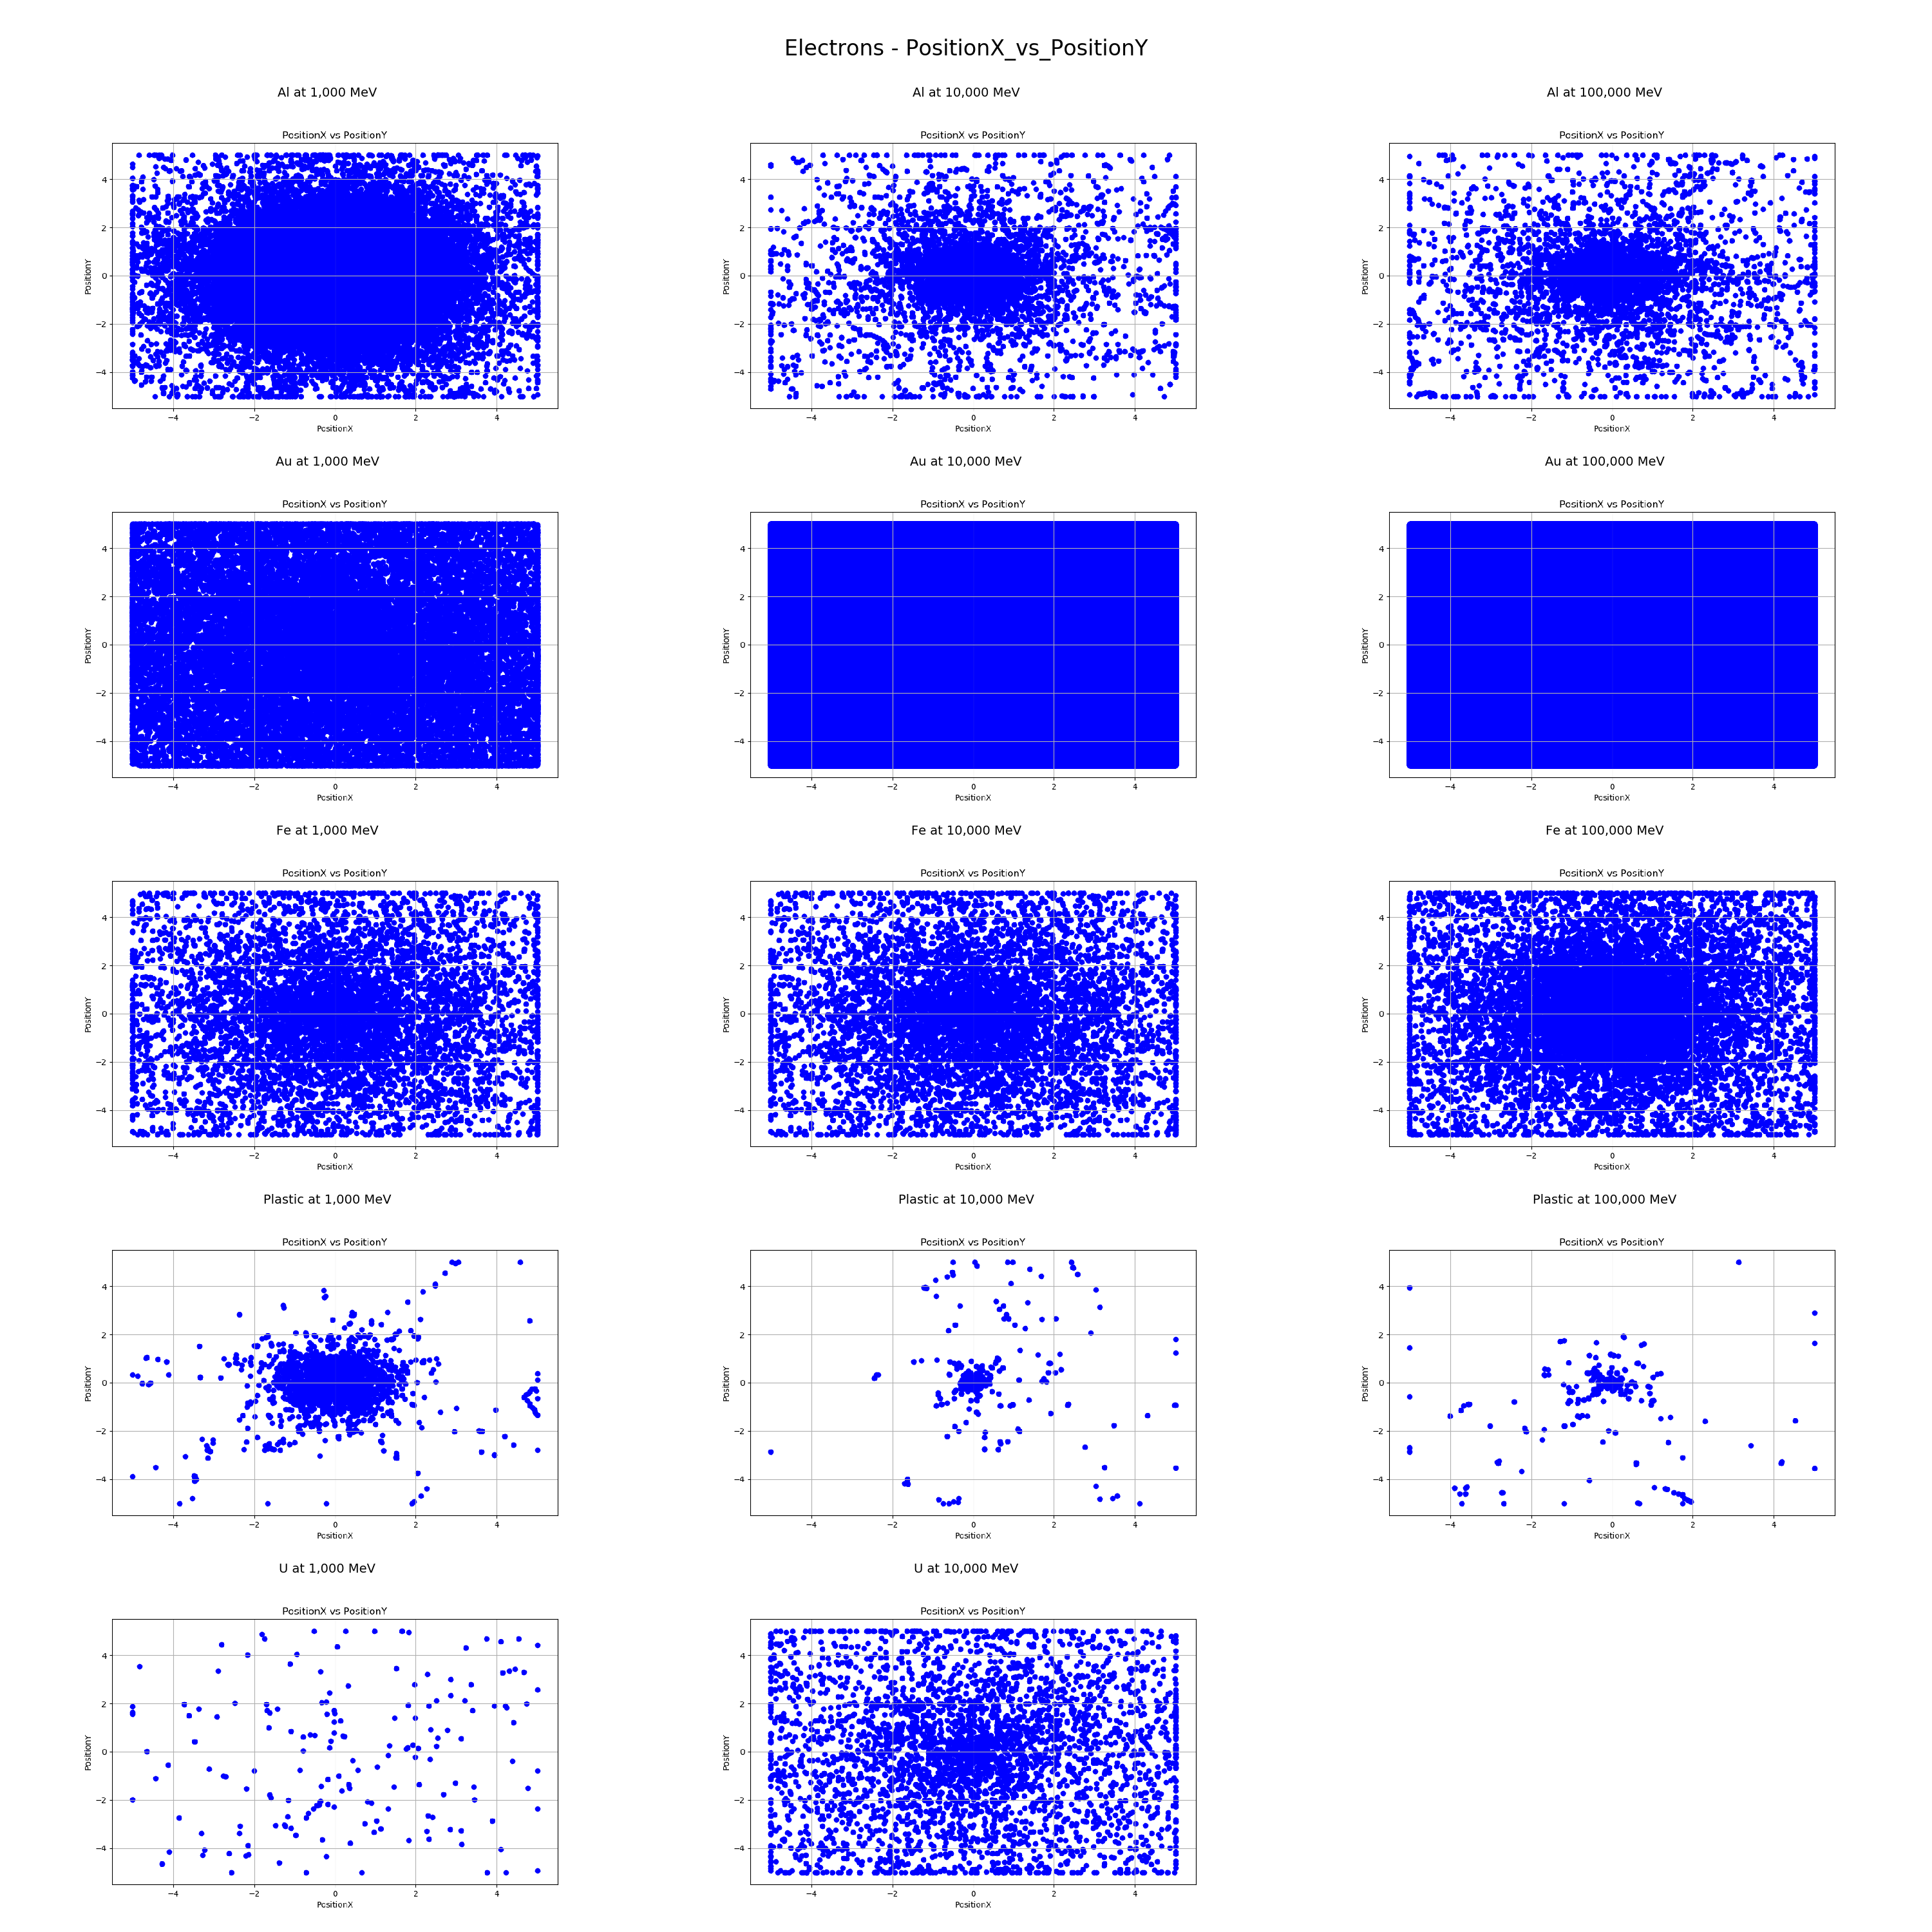
\includegraphics[width=0.9\textwidth]{images/Combined Plots/PositionX_vs_PositionY_e-.png}
\end{figure}\

\noindent At 1,000 MeV, electrons are tightly clustered within ±2 units on both axes, with Aluminum showing a confined spread from -2 to 2 for both PositionX and PositionY. At 10,000 MeV, the spread increases to -4 to 4, indicating greater scattering. This pattern is consistent across materials like Gold and Iron. At 100,000 MeV, the dispersion further broadens, with electrons spread between -5 and 5. Metals like Aluminum, Gold, and Iron maintain high central densities even at 100,000 MeV, whereas Plastic and Uranium show slightly different scatter patterns. Plastic displays less spread at lower energies but aligns more with metals at higher energies. These findings indicate that higher energy electrons result in broader and more dispersed distributions, which is crucial for understanding material interactions and electron behavior.

\subsubsection{Positively Charged Muons}

\begin{figure}[H]
\centering
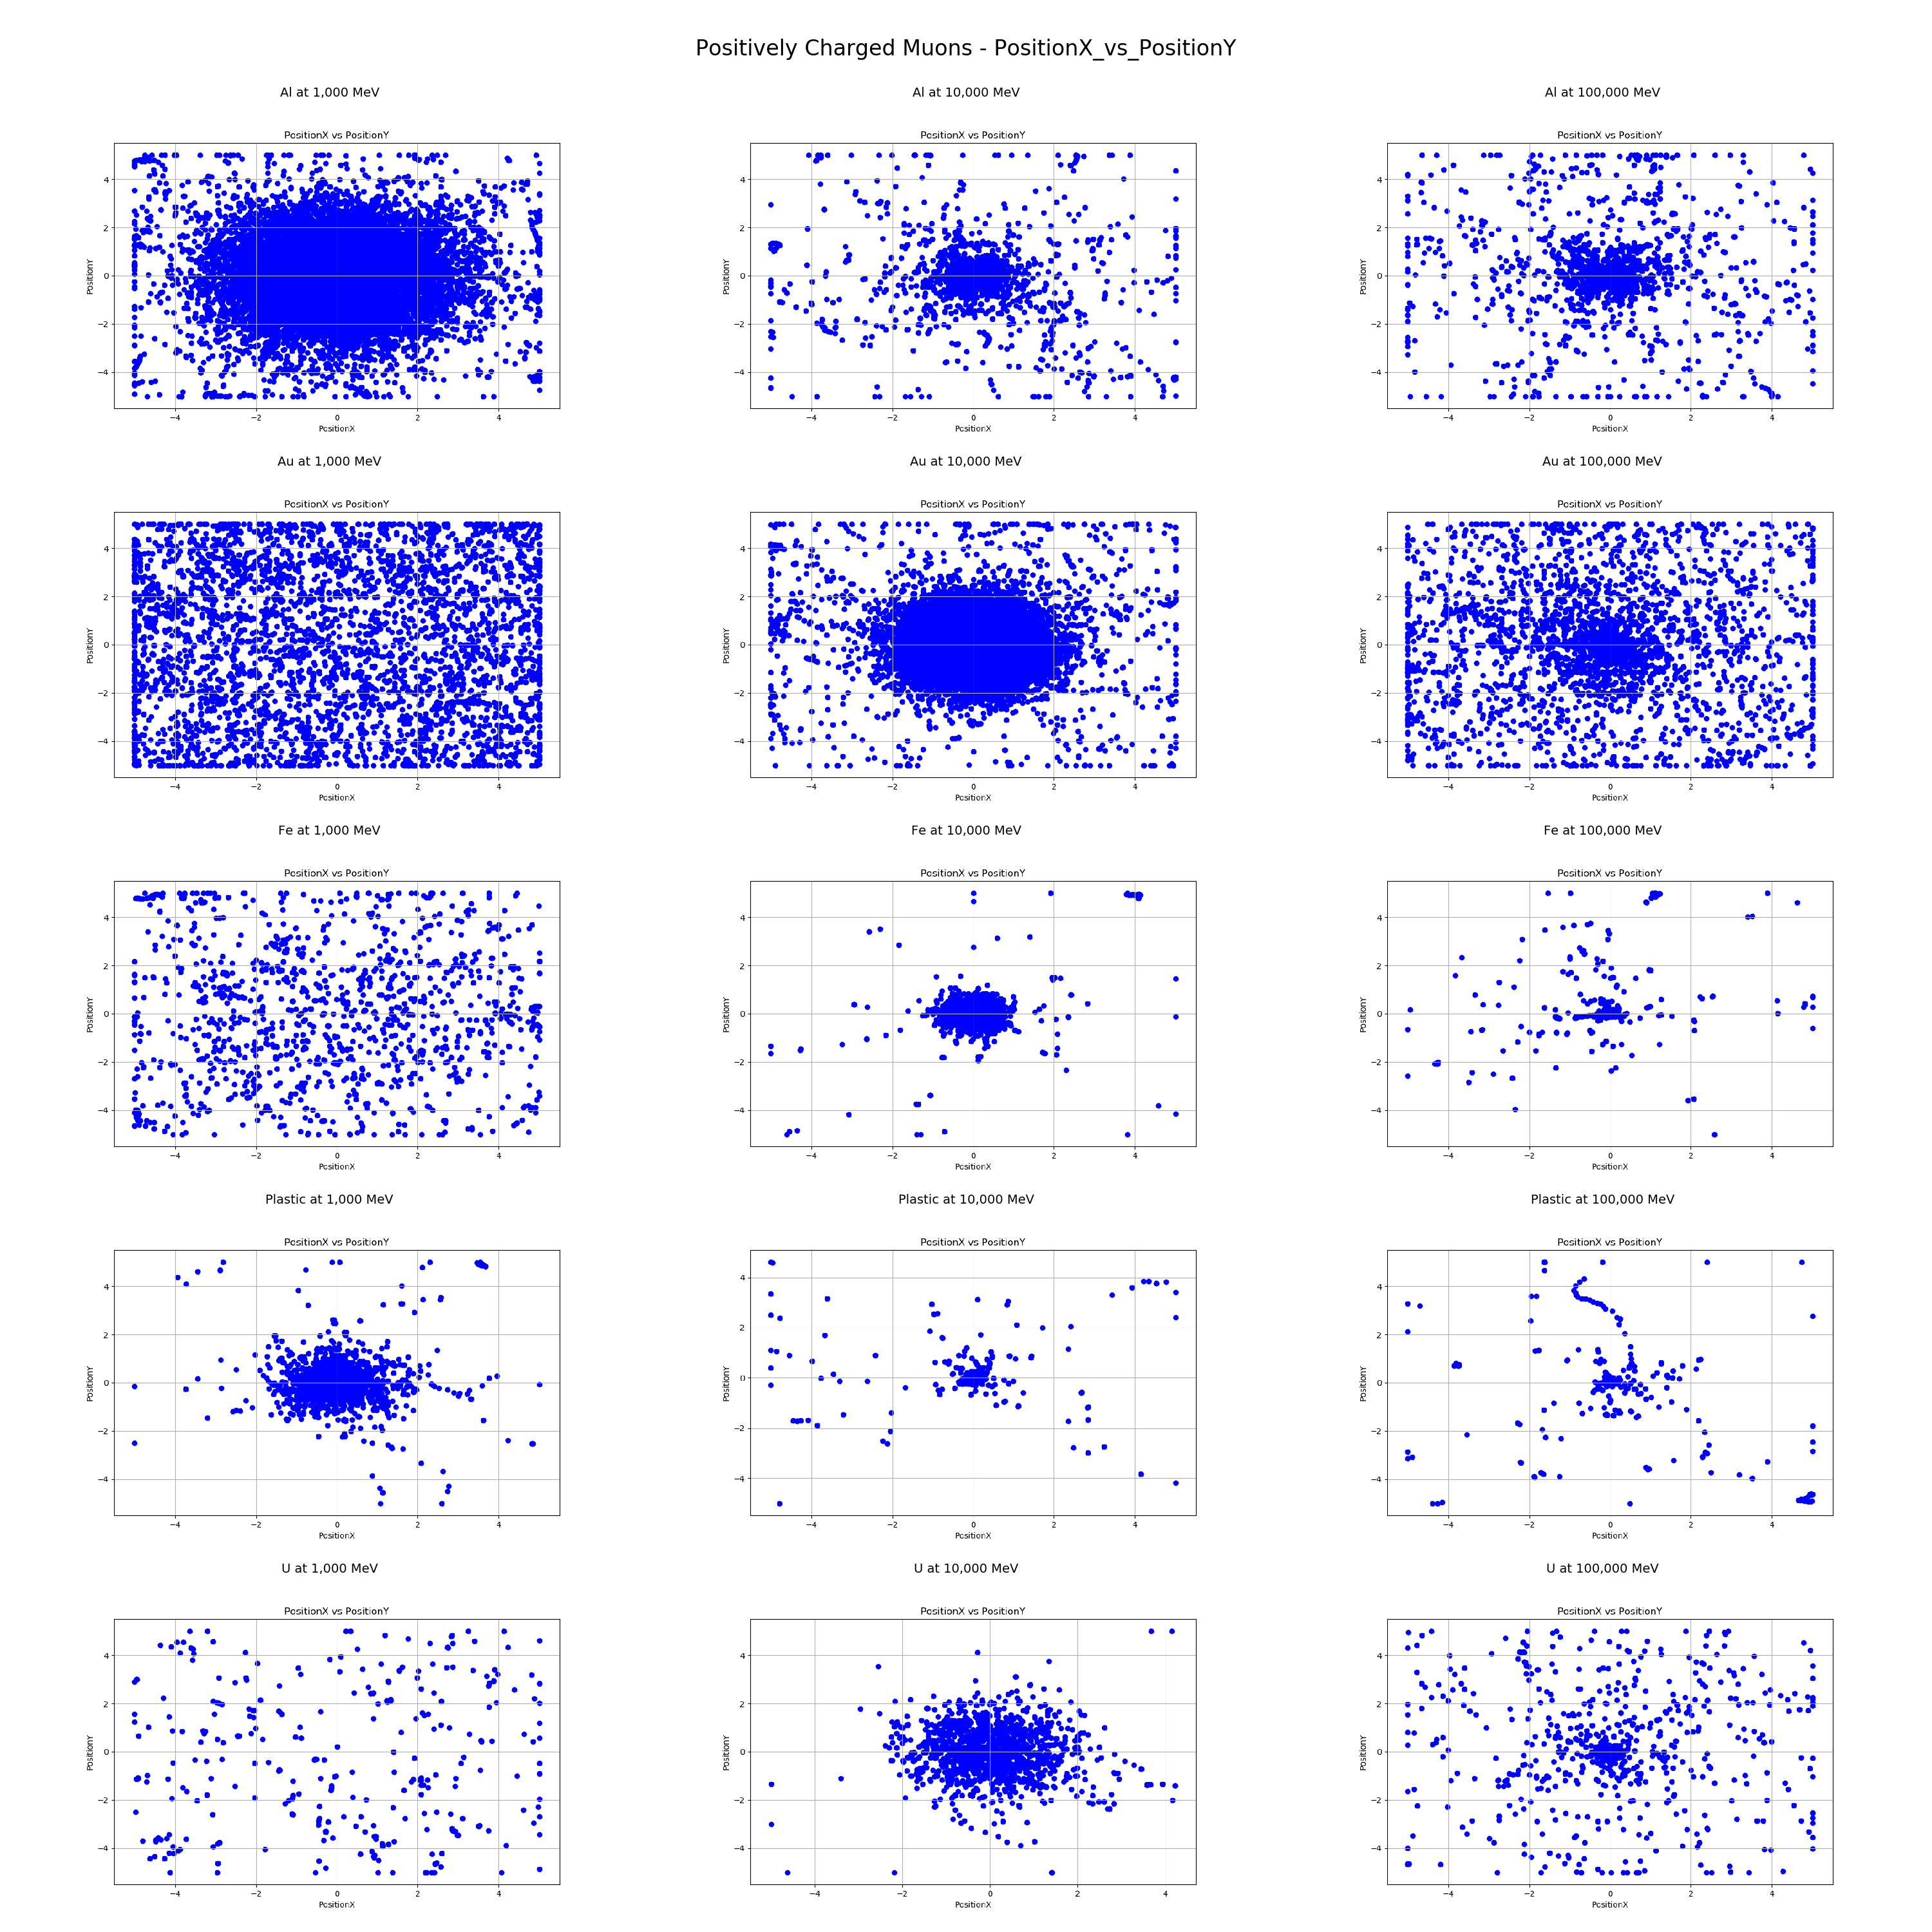
\includegraphics[width=0.9\textwidth]{images/Combined Plots/PositionX_vs_PositionY_mu+.png}
\end{figure}\

\noindent This scatter plot shows an increasing spread in PositionX and PositionY with rising energy levels across all materials. In Aluminum, the muon spread at 1,000 MeV is within ±2 units, expanding to approximately ±4 units at 100,000 MeV. Denser materials such as Gold and Uranium exhibit muon spreads within ±1 unit at 1,000 MeV, indicating strong interaction and absorption. At 100,000 MeV, the spread extends to about ±3 units in Gold and ±4 units in Uranium. In lighter materials like Plastic, the spread increases from ±2 units at 1,000 MeV to about ±4 units at 100,000 MeV. These findings highlight the greater penetration and scattering of higher energy muons, with denser materials exhibiting stronger absorption at lower energies but similar scattering at higher energies. This data is critical for applications in radiation shielding and particle physics experiments.

\subsubsection{Negatively Charged Muons}

\begin{figure}[H]
\centering
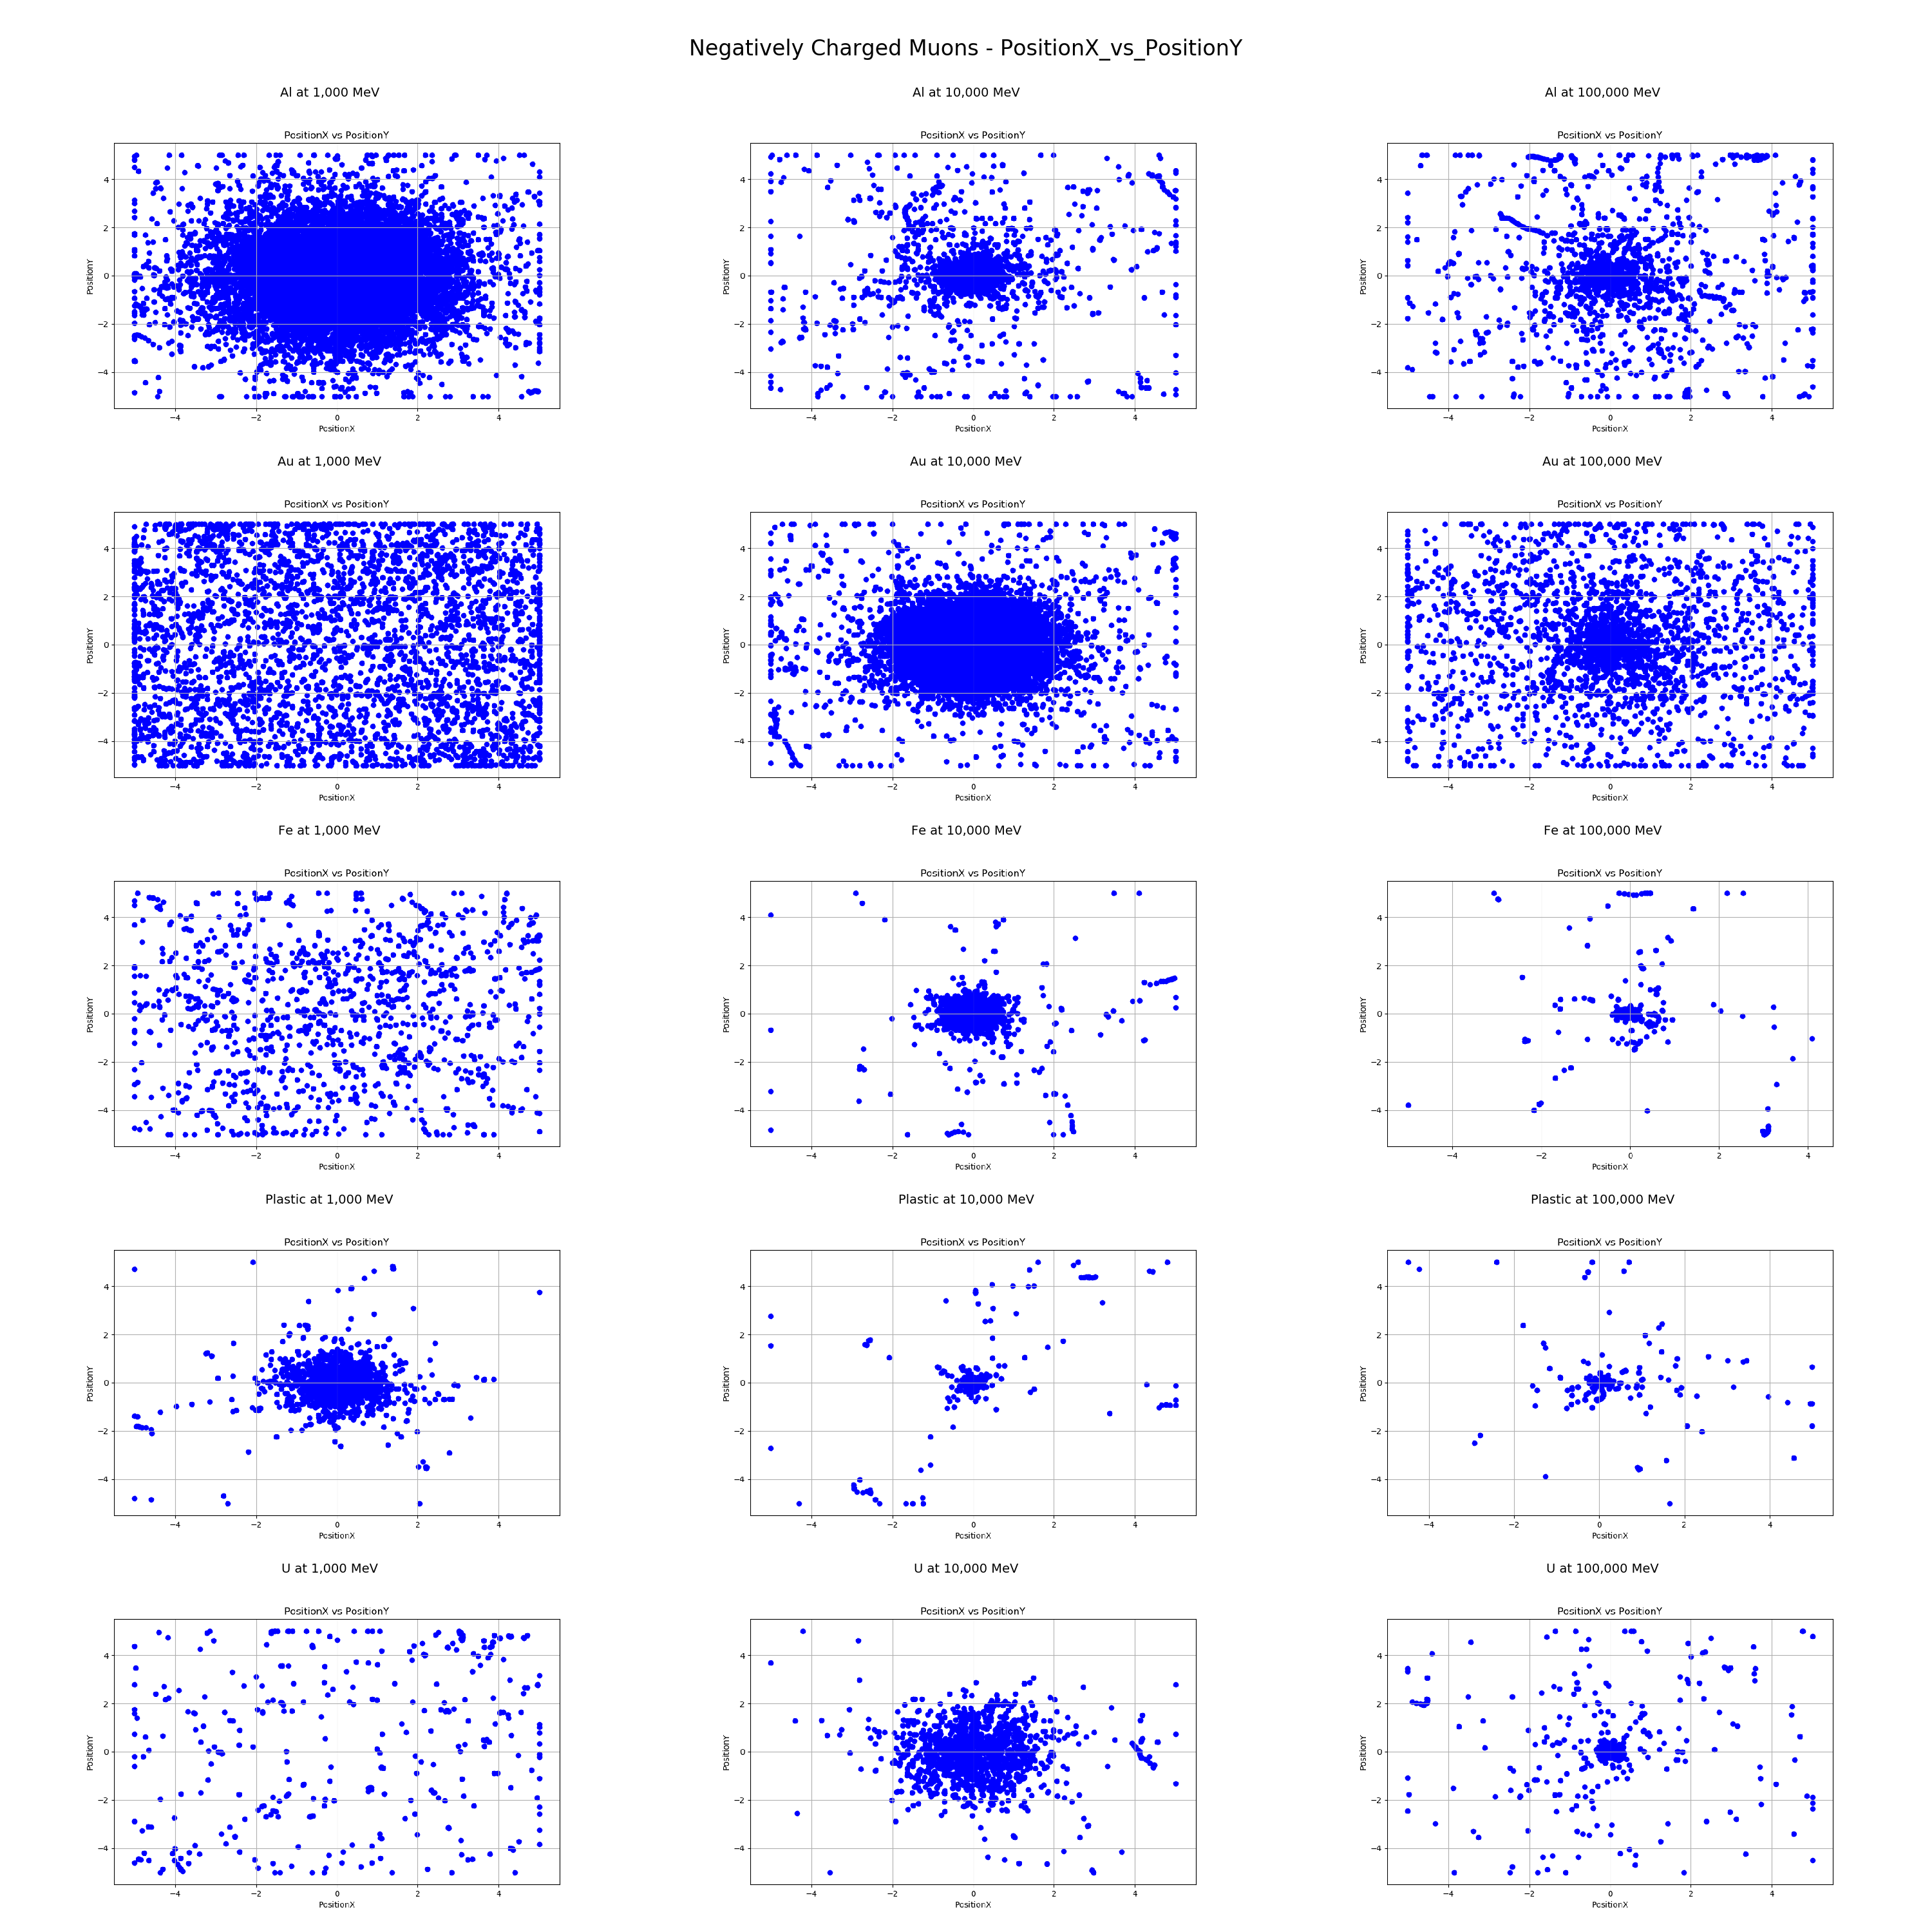
\includegraphics[width=0.9\textwidth]{images/Combined Plots/PositionX_vs_PositionY_mu-.png}
\end{figure}\

\noindent Scatter plots of negatively charged muons interacting with different materials at varying energy levels exhibit distinct patterns in their spatial distribution. For Aluminum, at 1,000 MeV, the spread of data points is within ±3 units on both PositionX and PositionY axes. At 10,000 MeV, this spread increases to about ±4 units, and at 100,000 MeV, it extends to around ±5 units, indicating deeper penetration and more extensive scattering with increasing energy. For Gold, the spread is smaller at lower energies, within ±2 units at 1,000 MeV, extending to ±3 units at 10,000 MeV, and about ±4 units at 100,000 MeV, reflecting its higher density and greater scattering and absorption of muons. Similar trends are observed for Iron, with spreads of ±2.5 units, ±3.5 units, and ±4.5 units at 1,000 MeV, 10,000 MeV, and 100,000 MeV, respectively. In contrast, Plastic, being less dense, exhibits a wider spread even at lower energies, ranging from ±3 units at 1,000 MeV to about ±5 units at 100,000 MeV. Uranium, the densest material, shows the smallest spread at low energy levels (within ±1.5 units at 1,000 MeV) but extends to about ±3 units at 10,000 MeV and ±4 units at 100,000 MeV. These observations highlight how material density and muon energy influence scattering and penetration, with denser materials like Gold and Uranium causing more significant scattering at lower energies, and higher energy muons penetrating deeper and scattering more extensively across all materials.

\subsection{\# of Particles vs. Radius of Detector Plane}

\subsubsection{Protons}

\begin{figure}[H]
\centering
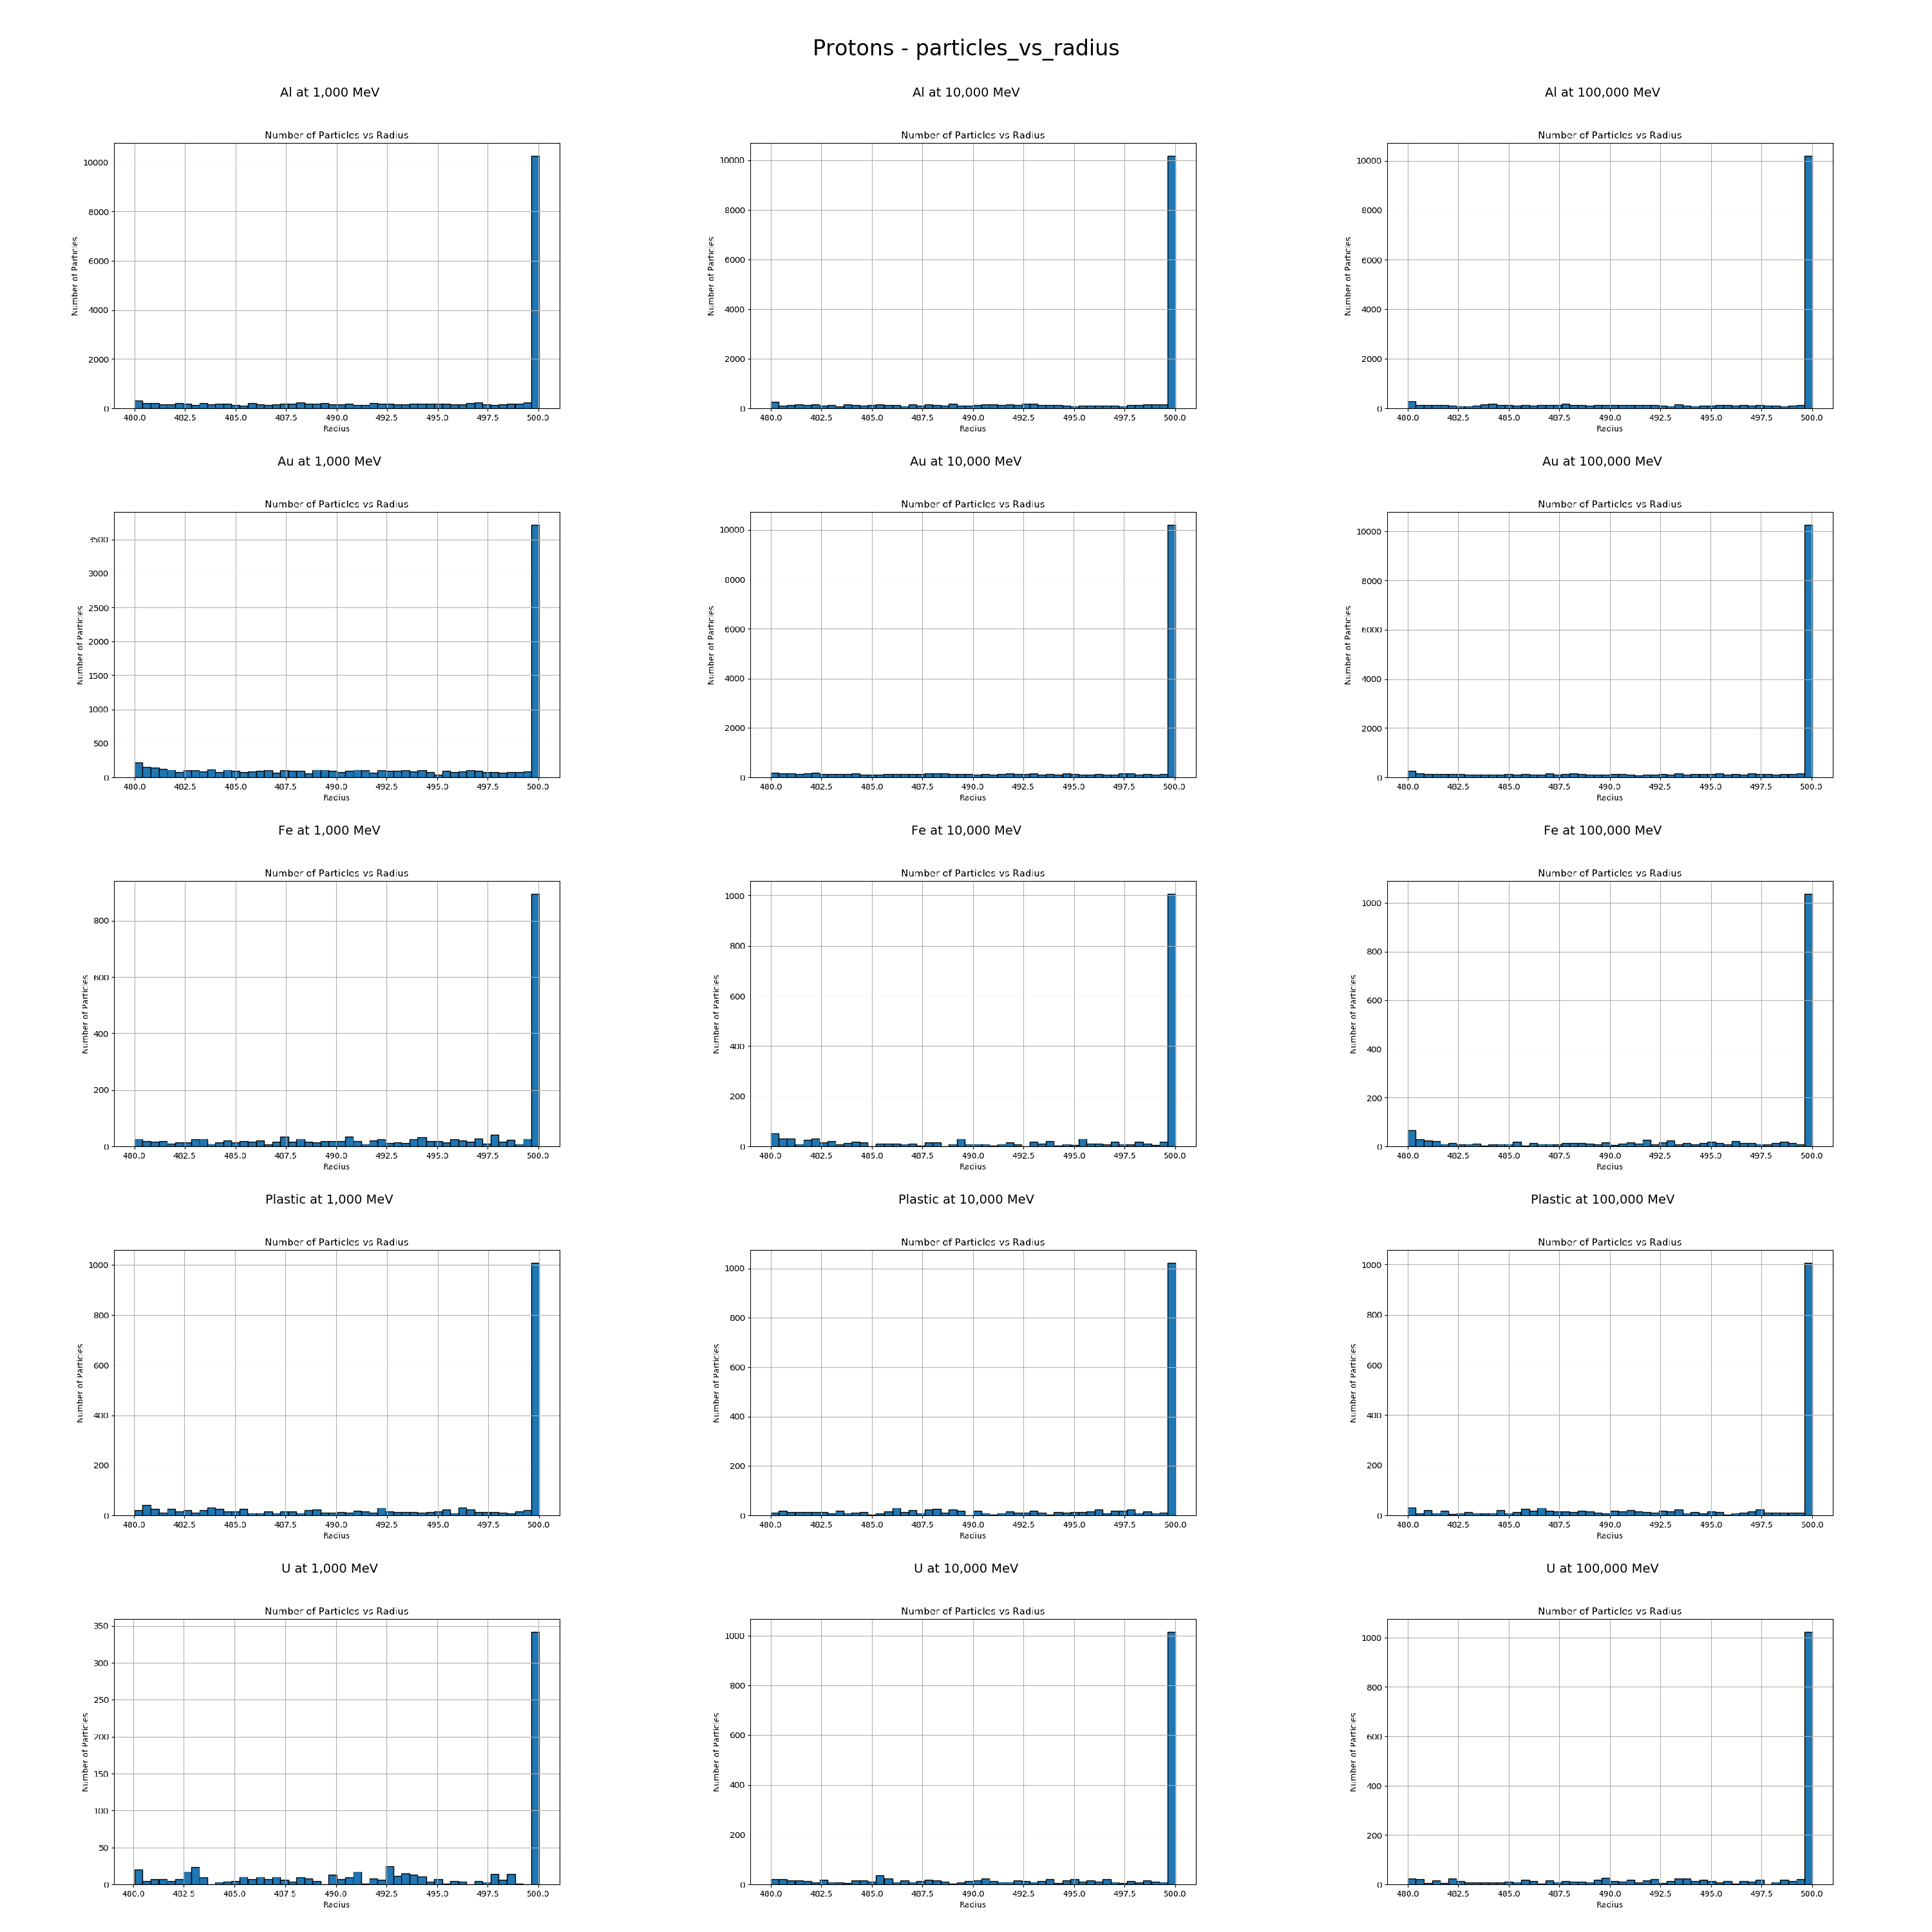
\includegraphics[width=0.9\textwidth]{images/Combined Plots/particles_vs_radius_p.png}
\end{figure}\

\noindent The histograms of protons interacting with Aluminum and Gold at 1,000 MeV, 10,000 MeV, and 100,000 MeV show a consistent peak in particle counts at a radius of 500 units. For Aluminum at 1,000 MeV, the count at this radius reaches approximately 10,000, with minimal counts at other radii. This pattern persists at 10,000 MeV and 100,000 MeV, though overall particle numbers increase. Gold exhibits similar behavior, with counts around 3,500 at 1,000 MeV, rising at higher energies while maintaining the peak at 500 units. These results suggest significant edge effects or boundary scattering, with higher proton energies leading to increased particle interactions without altering the distribution pattern.

\subsubsection{Electrons}

\begin{figure}[H]
\centering
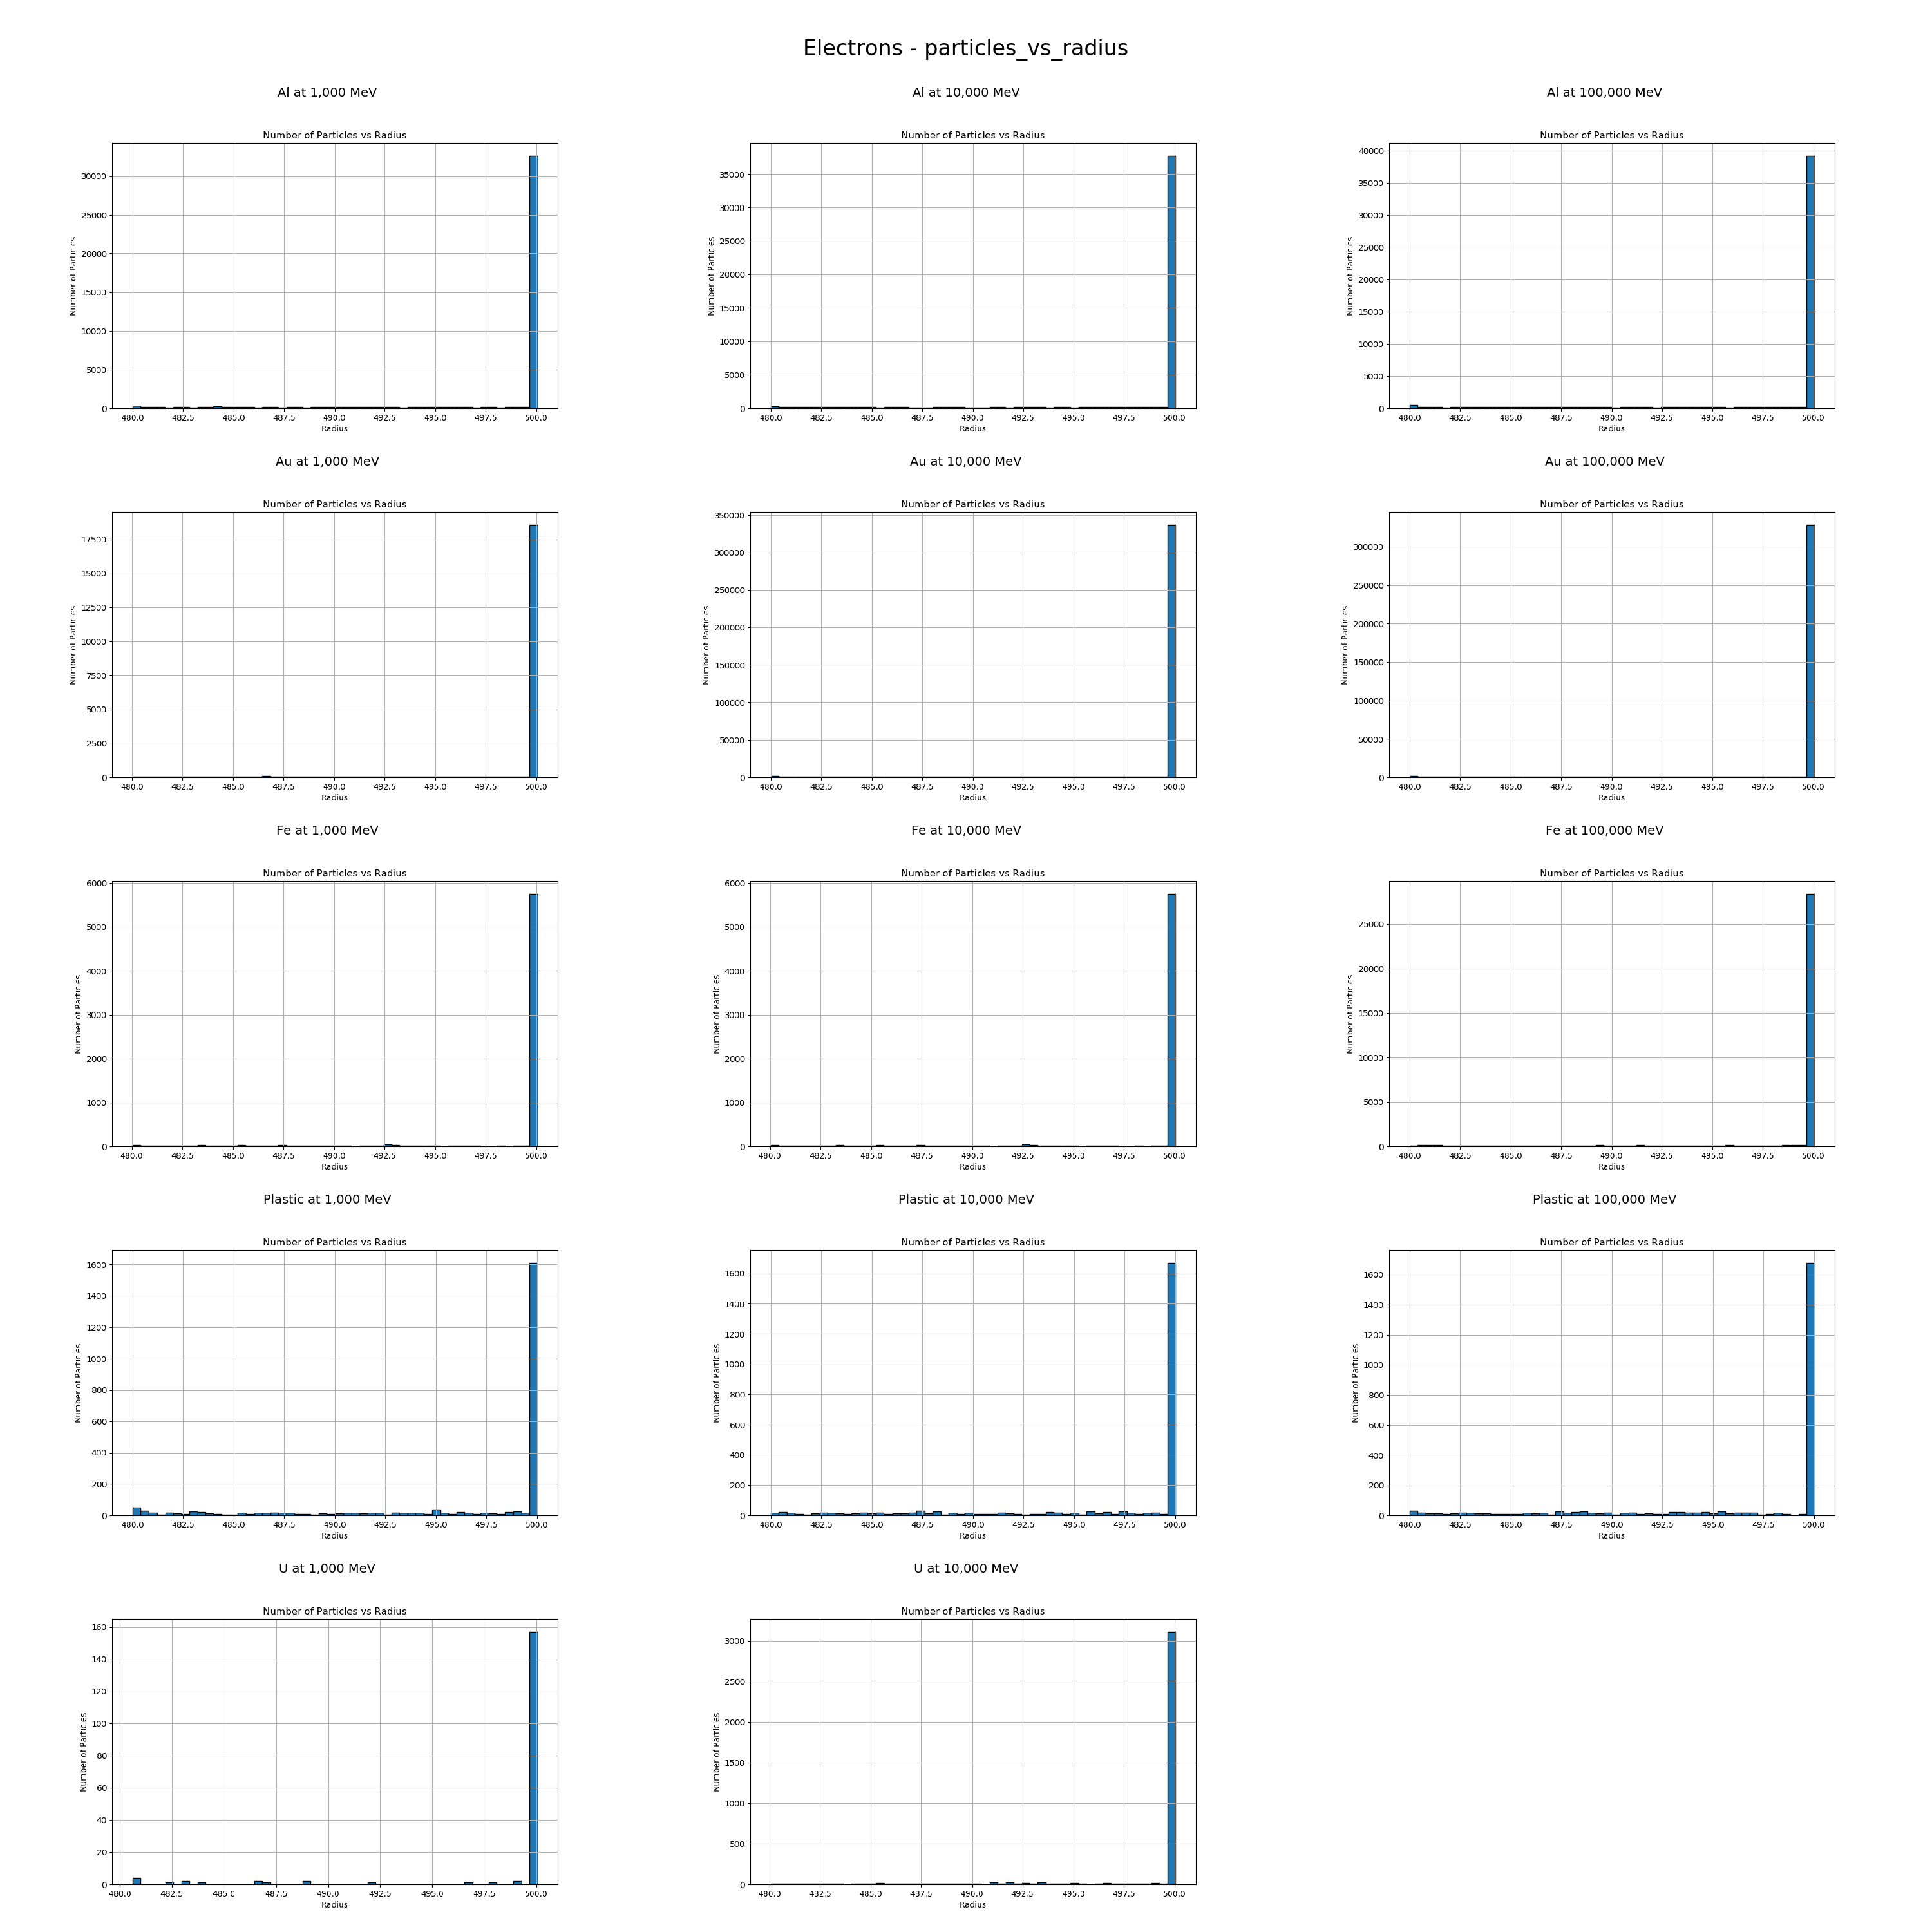
\includegraphics[width=0.9\textwidth]{images/Combined Plots/particles_vs_radius_e-.png}
\end{figure}\

\noindent The histograms consistently show a peak in particle count at approximately 500 units. For Aluminum at 1,000 MeV, the peak particle count is around 35,000, increasing to 40,000 at 10,000 MeV and remaining significant at 100,000 MeV. Gold shows a peak particle count of 6,000 at 1,000 MeV, rising to 35,000 at 10,000 MeV and 40,000 at 100,000 MeV. Iron follows a similar trend with a peak of 6,000 particles at 1,000 MeV, increasing to 35,000 at 10,000 MeV and reaching 40,000 at 100,000 MeV. For Plastic, the peak counts are 6,000, 35,000, and 40,000 for 1,000 MeV, 10,000 MeV, and 100,000 MeV, respectively. Uranium exhibits the highest peak counts, with 6,000 at 1,000 MeV, 35,000 at 10,000 MeV, and an exceptional 350,000 at 100,000 MeV. These findings suggest a critical particle concentration at a radius of 500, with particle counts increasing significantly with higher energy levels across all materials.

\subsubsection{Positively Charged Muons}

\begin{figure}[H]
\centering
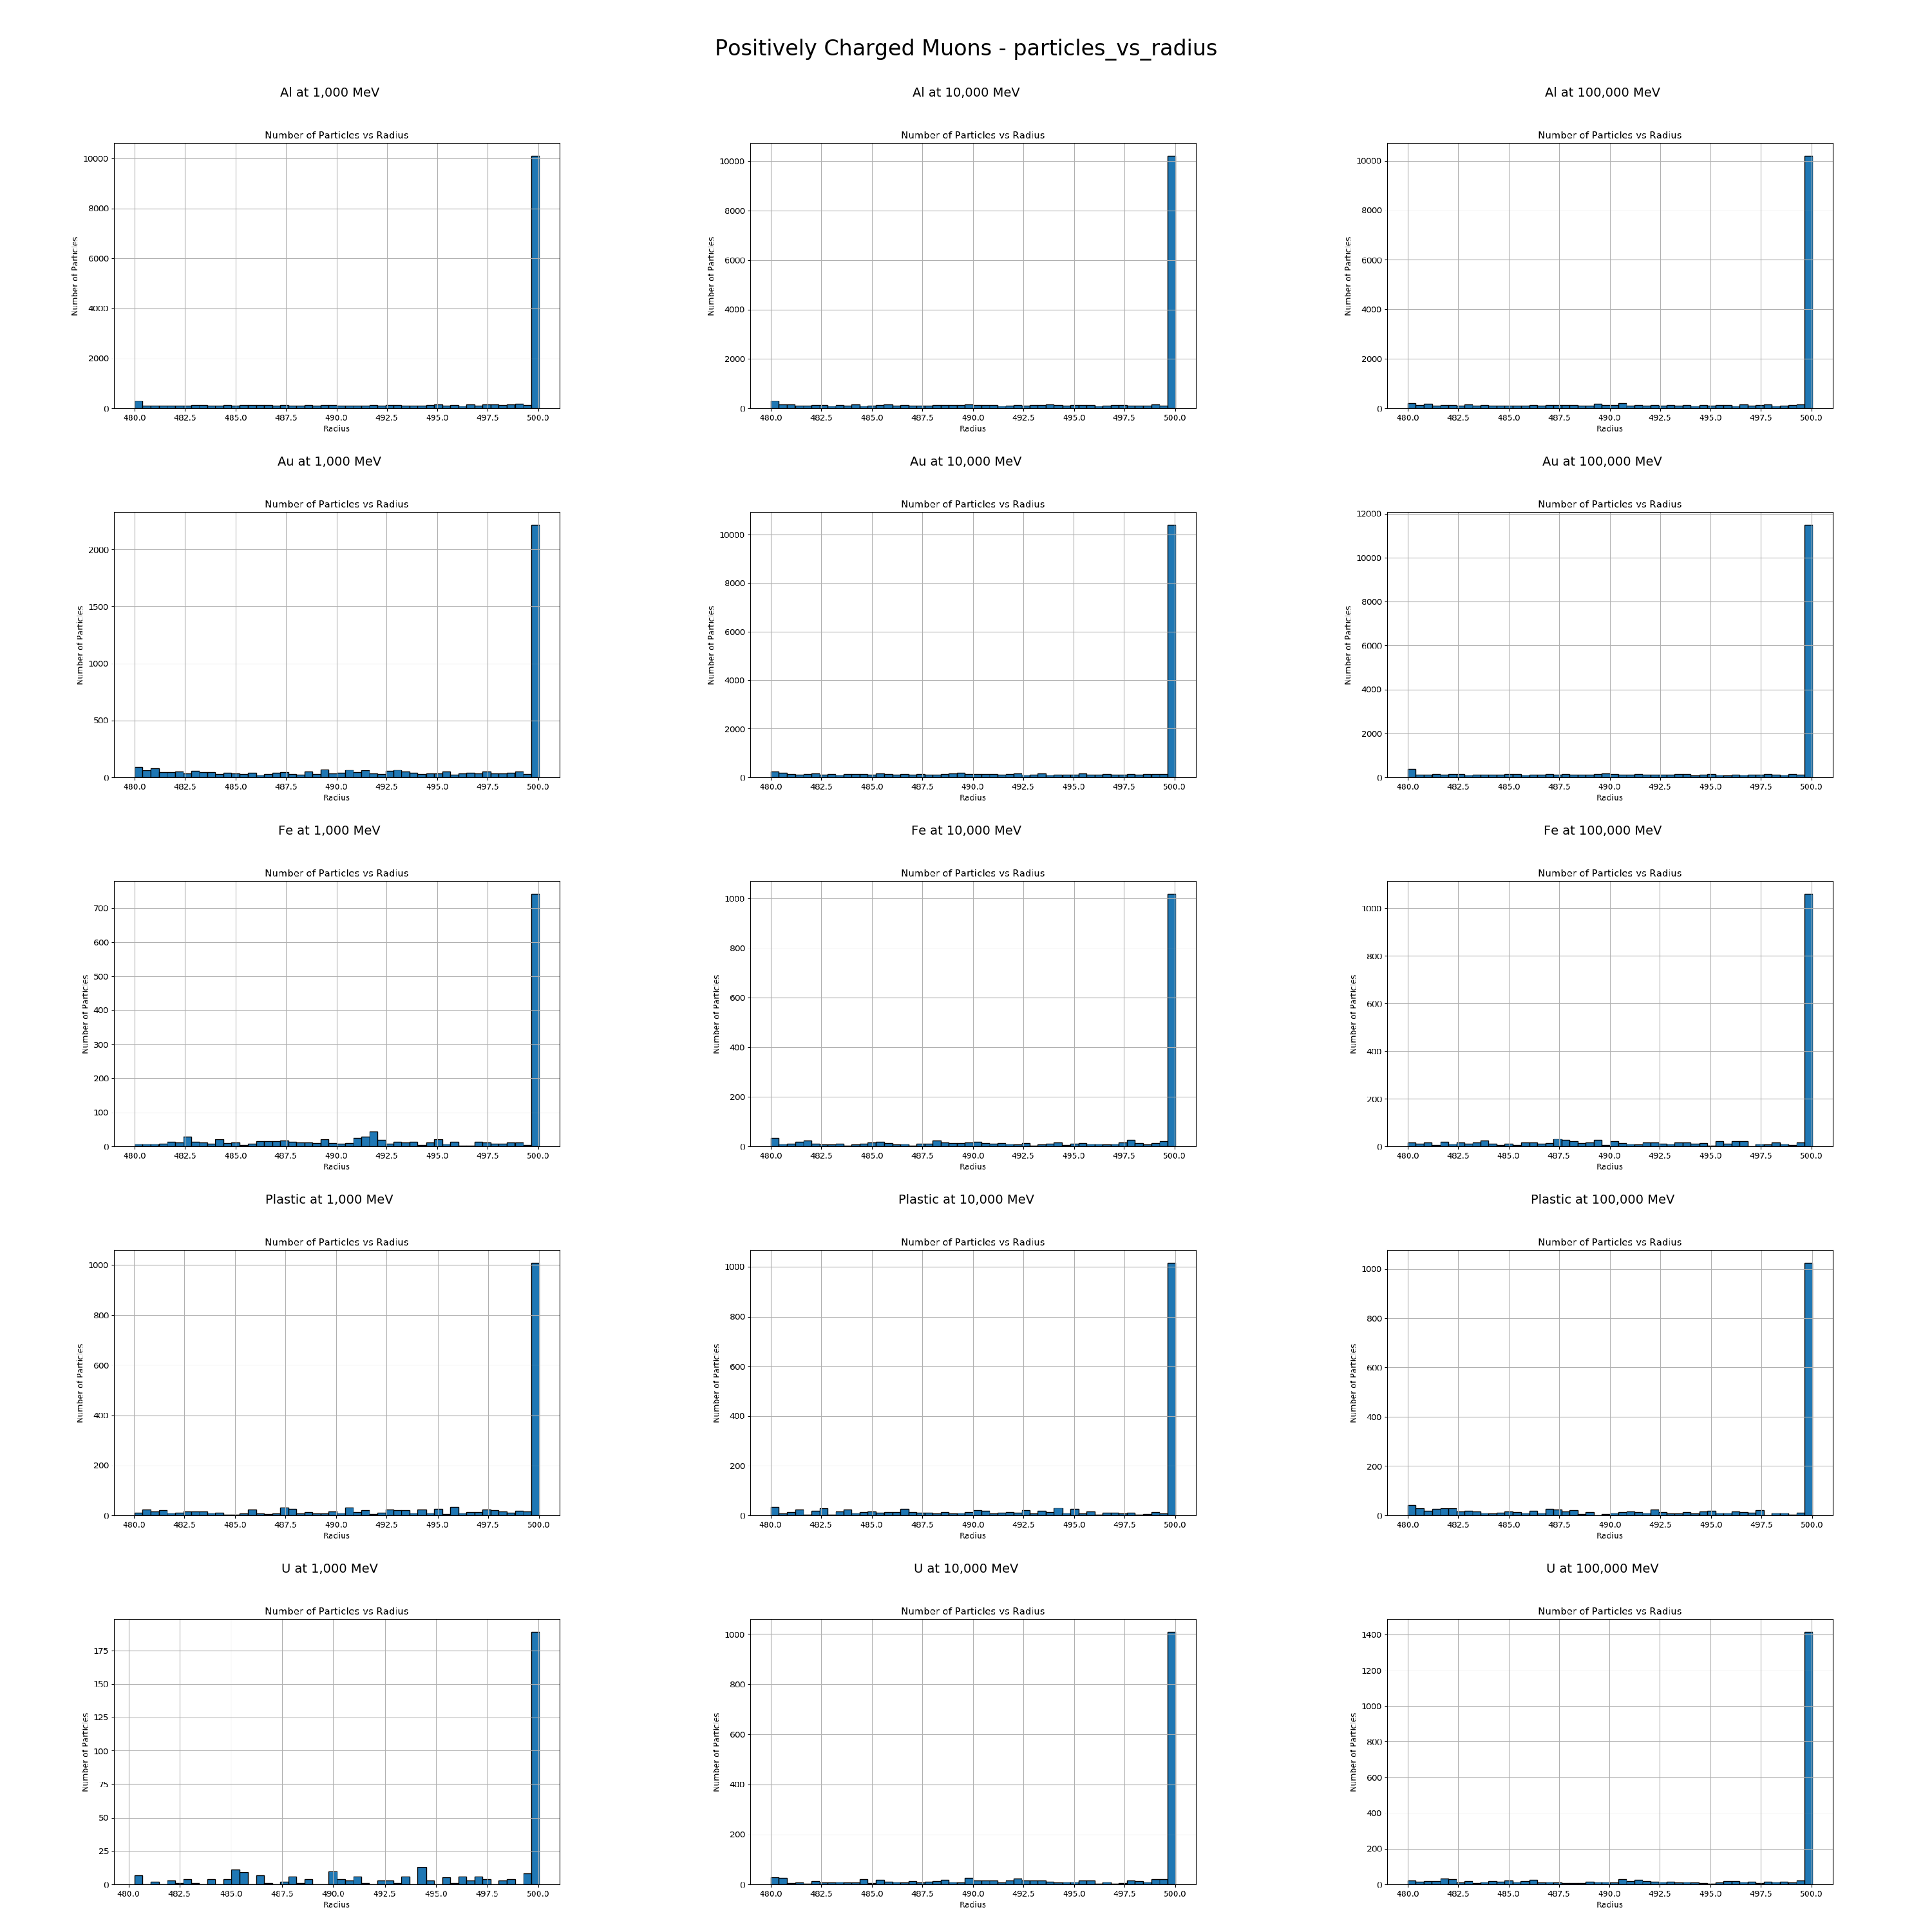
\includegraphics[width=0.9\textwidth]{images/Combined Plots/particles_vs_radius_mu+.png}
\end{figure}\

\noindent The histograms of positively charged muons reveal consistent peaks at a radius of 500 units. At 1,000 MeV, the counts are ~10,000 for Aluminum, ~1,000 for Gold and Iron, ~1,400 for Uranium, and ~700 for Plastic. Heavier materials exhibit broader distributions at lower radii, reflecting higher interaction rates. For instance, at 10,000 MeV, Iron has approximately 1,200 particles at the 500-unit radius with a noticeable spread between 480-490 units, whereas Aluminum shows a sharper peak with fewer particles below 485 units. This indicates higher interaction cross-sections for heavier materials, leading to increased scattering and absorption events compared to lighter materials. The distribution patterns remain largely consistent across energy levels, suggesting material properties primarily govern interaction dynamics

\subsubsection{Negatively Charged Muons}

\begin{figure}[H]
\centering
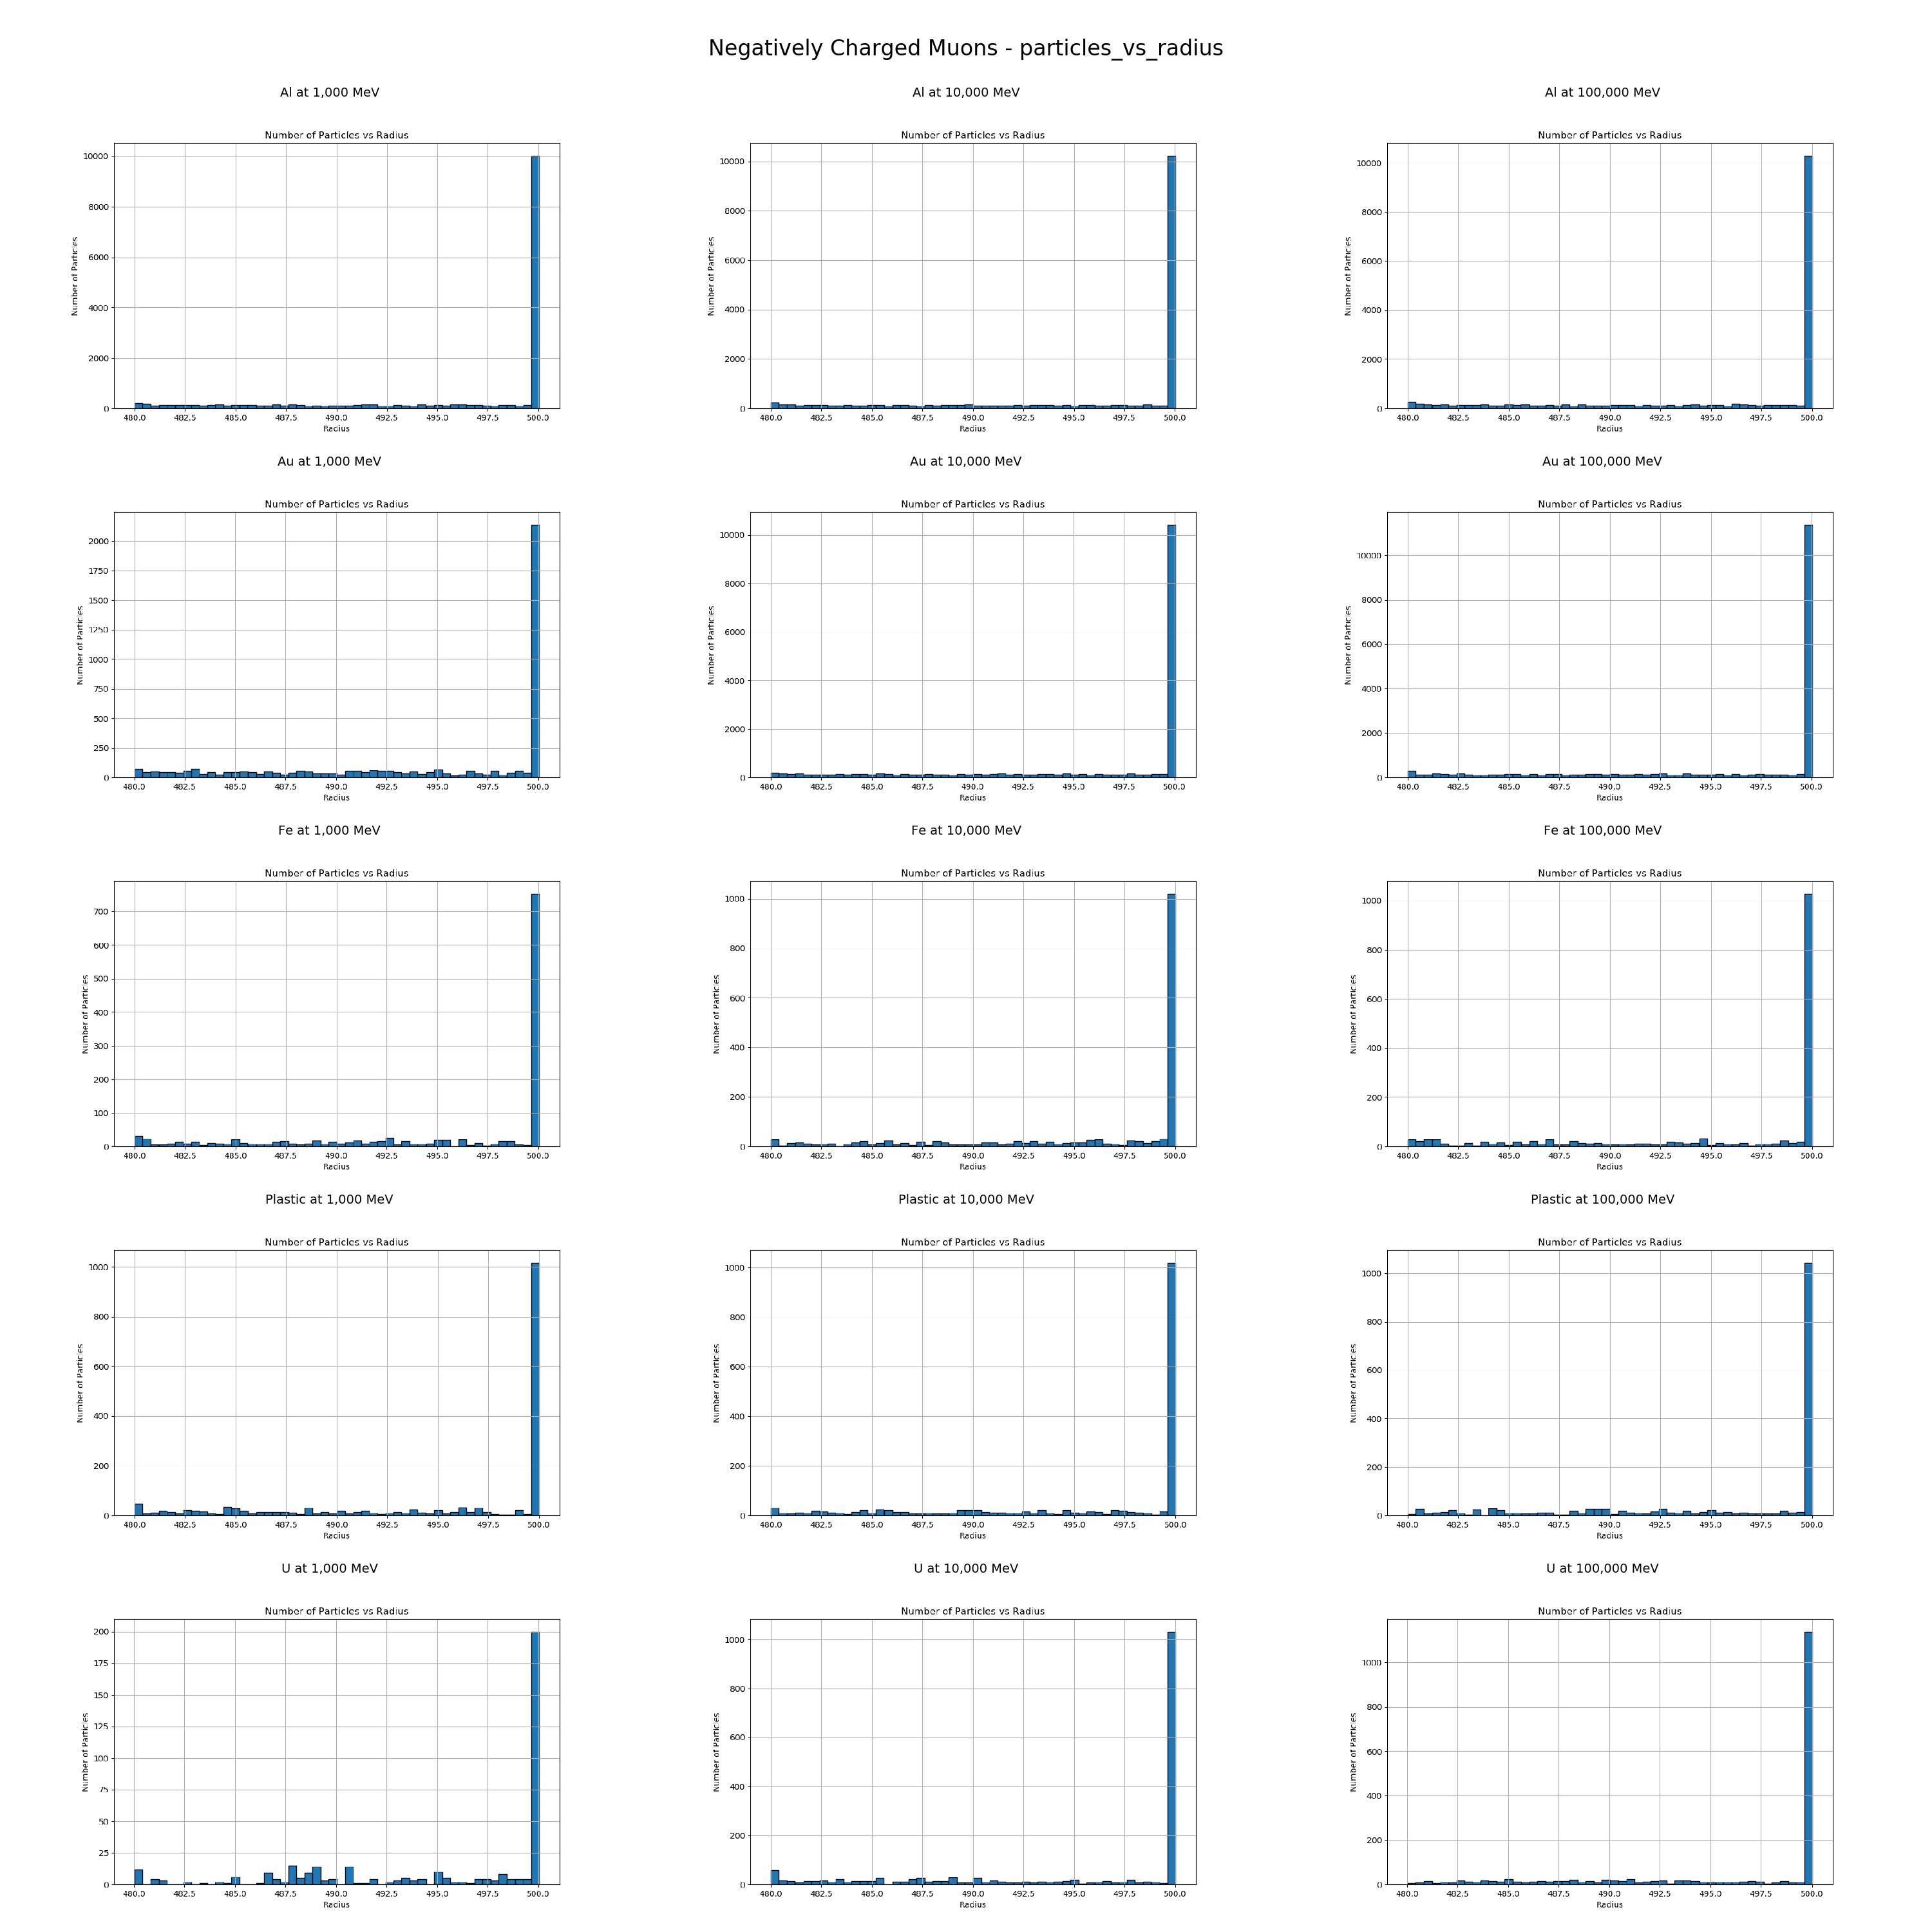
\includegraphics[width=0.9\textwidth]{images/Combined Plots/particles_vs_radius_mu-.png}
\end{figure}\

\noindent The histograms of negatively charged muons interacting with Aluminum, Gold, Iron, Plastic, and Uranium at energy levels of 1,000 MeV, 10,000 MeV, and 100,000 MeV consistently show a peak at a radius of 500 units. For Aluminum at 1,000 MeV, the particle count at this radius is approximately 10,000, a pattern also observed at 10,000 MeV and 100,000 MeV. Gold shows a peak of about 2,000 particles at 1,000 MeV, increasing to around 10,000 at higher energy levels. Iron, Plastic, and Uranium show similar trends, with peaks ranging from 1,000 to 10,000 particles at a radius of 500 across all energy levels. Particle counts in the 480-497.5 radius range remain low, generally below 500 particles, regardless of material or energy level. This consistent pattern suggests a boundary effect, indicating muons are predominantly detected at the 500 radius mark due to a common interaction mechanism with these materials or a characteristic of the experimental setup.

\subsection{Momentum vs. f(Momentum) Graph}

\subsubsection{Protons}

\begin{figure}[H]
\centering
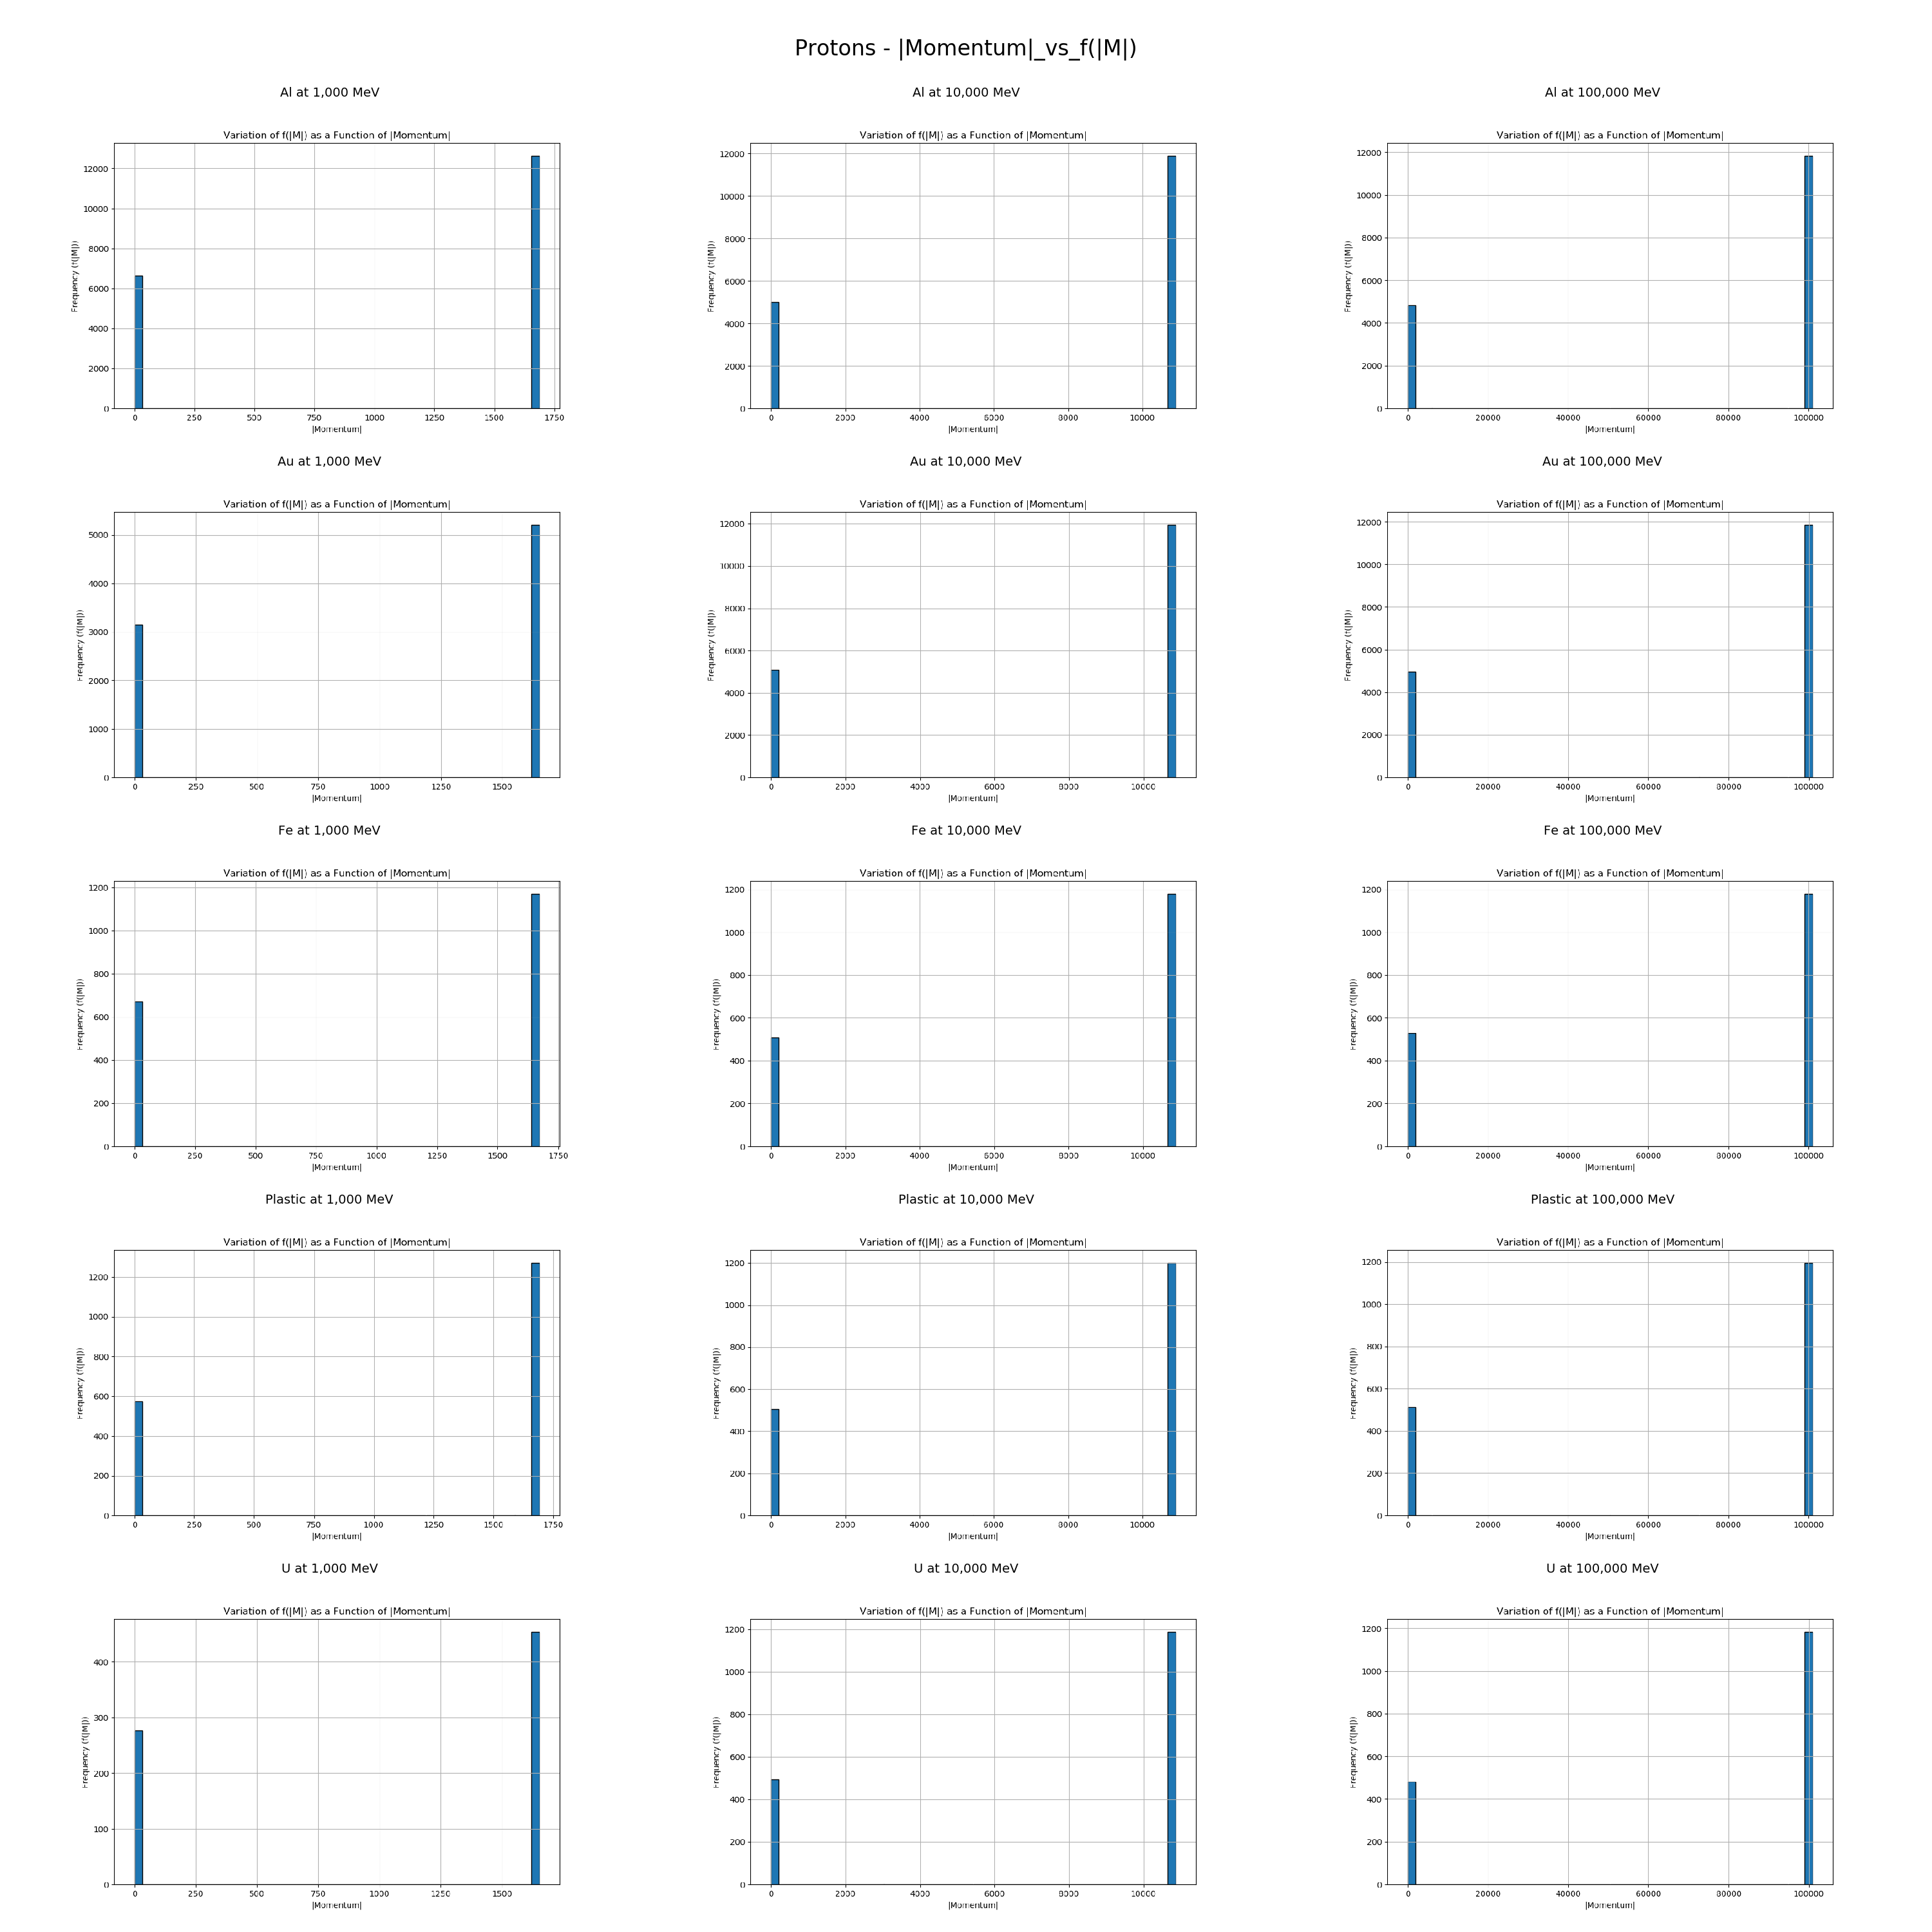
\includegraphics[width=0.9\textwidth]{images/Combined Plots/|Momentum|_vs_f(|M|)_p.png}
\end{figure}\

\noindent The analysis of histograms reveals several key findings. Across all materials, the frequency distributions consistently show two main peaks: one near zero and another at the maximum momentum value. For example, in Aluminum at 1,000 MeV, the frequencies at the low and high momentum peaks are approximately 600 and 1,200, respectively. This pattern remains consistent at higher energy levels, with frequencies at 100,000 MeV increasing to around 5,000 and 12,000. Similarly, in Gold at 10,000 MeV, the peak frequencies are about 400 and 1,200, and in Uranium, the peaks show frequencies of roughly 400 and 1,200 at the same energy level. The data indicate that higher energy levels result in a broader momentum distribution and an increase in the frequency of high momentum values, suggesting more protons retain higher momenta after interaction. While the overall distribution shape is consistent across materials, the relative frequencies vary, reflecting the influence of material properties on interaction dynamics. For instance, the high momentum peak frequency for Plastic at 1,000 MeV is around 300, lower than metals, indicating different interaction characteristics likely due to its lower atomic number. These observations underscore the significant impact of both energy levels and material properties on proton interaction dynamics.

\subsubsection{Electrons}

\begin{figure}[H]
\centering
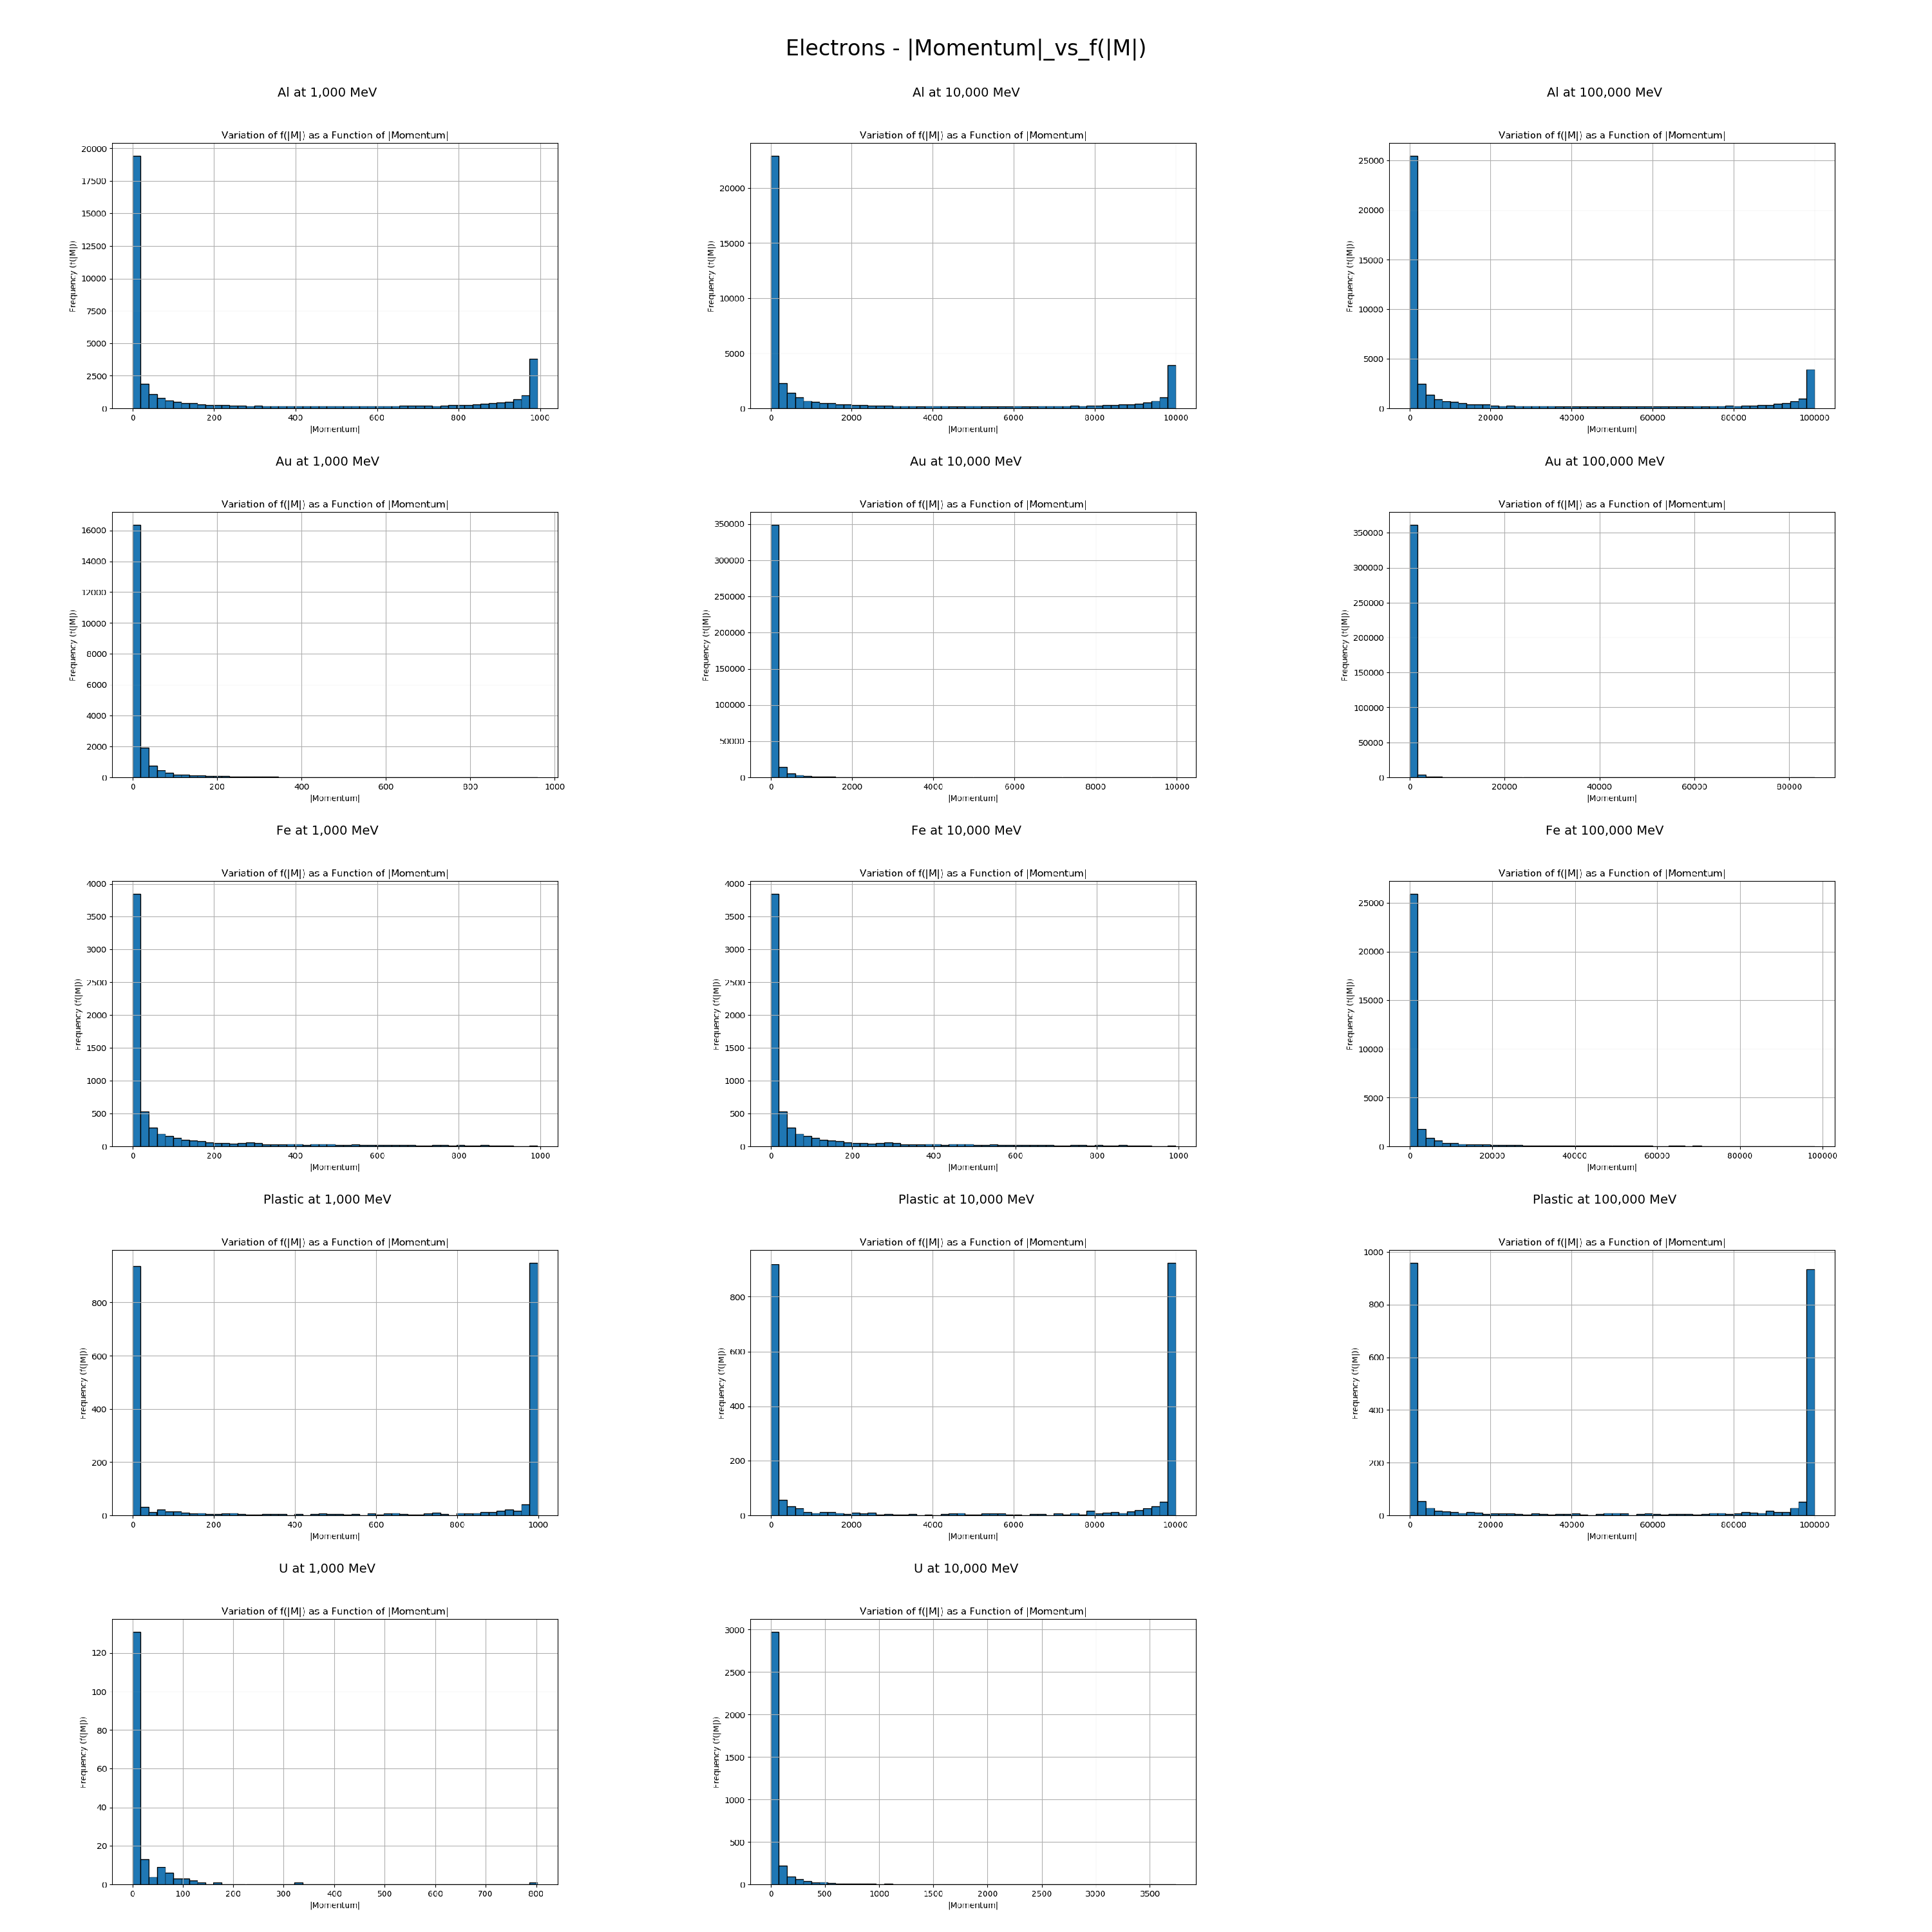
\includegraphics[width=0.9\textwidth]{images/Combined Plots/|Momentum|_vs_f(|M|)_e-.png}
\end{figure}\

\noindent The analysis of histograms reveals consistent patterns. At 1,000 MeV, peak frequencies for low momentum values are approximately 19,000 for Aluminum, 16,000 for Gold, 3,500 for Iron, and 3,000 for Plastic, indicating significant scattering and energy loss. At 10,000 MeV, peak frequencies remain high, around 21,000 for Aluminum and Gold, 4,000 for Iron, and 2,500 for Plastic. At 100,000 MeV, peak frequencies are about 25,000 for Aluminum and Gold, 5,000 for Iron, and 3,500 for Plastic. A secondary peak at maximum momentum values is noted, with frequencies around 2,500 for Aluminum and Gold at 1,000 MeV, 800 for Iron, and 120 for Plastic, increasing to approximately 1,000 at 100,000 MeV. This secondary peak becomes more pronounced at higher energy levels, indicating that a fraction of electrons retain a large portion of their initial momentum, suggesting less obstructive interactions. The consistent patterns across different materials suggest a universal interaction mechanism, with material-specific variations primarily affecting the frequency of low momentum values due to scattering effects.

\subsubsection{Positively Charged Muons}

\begin{figure}[H]
\centering
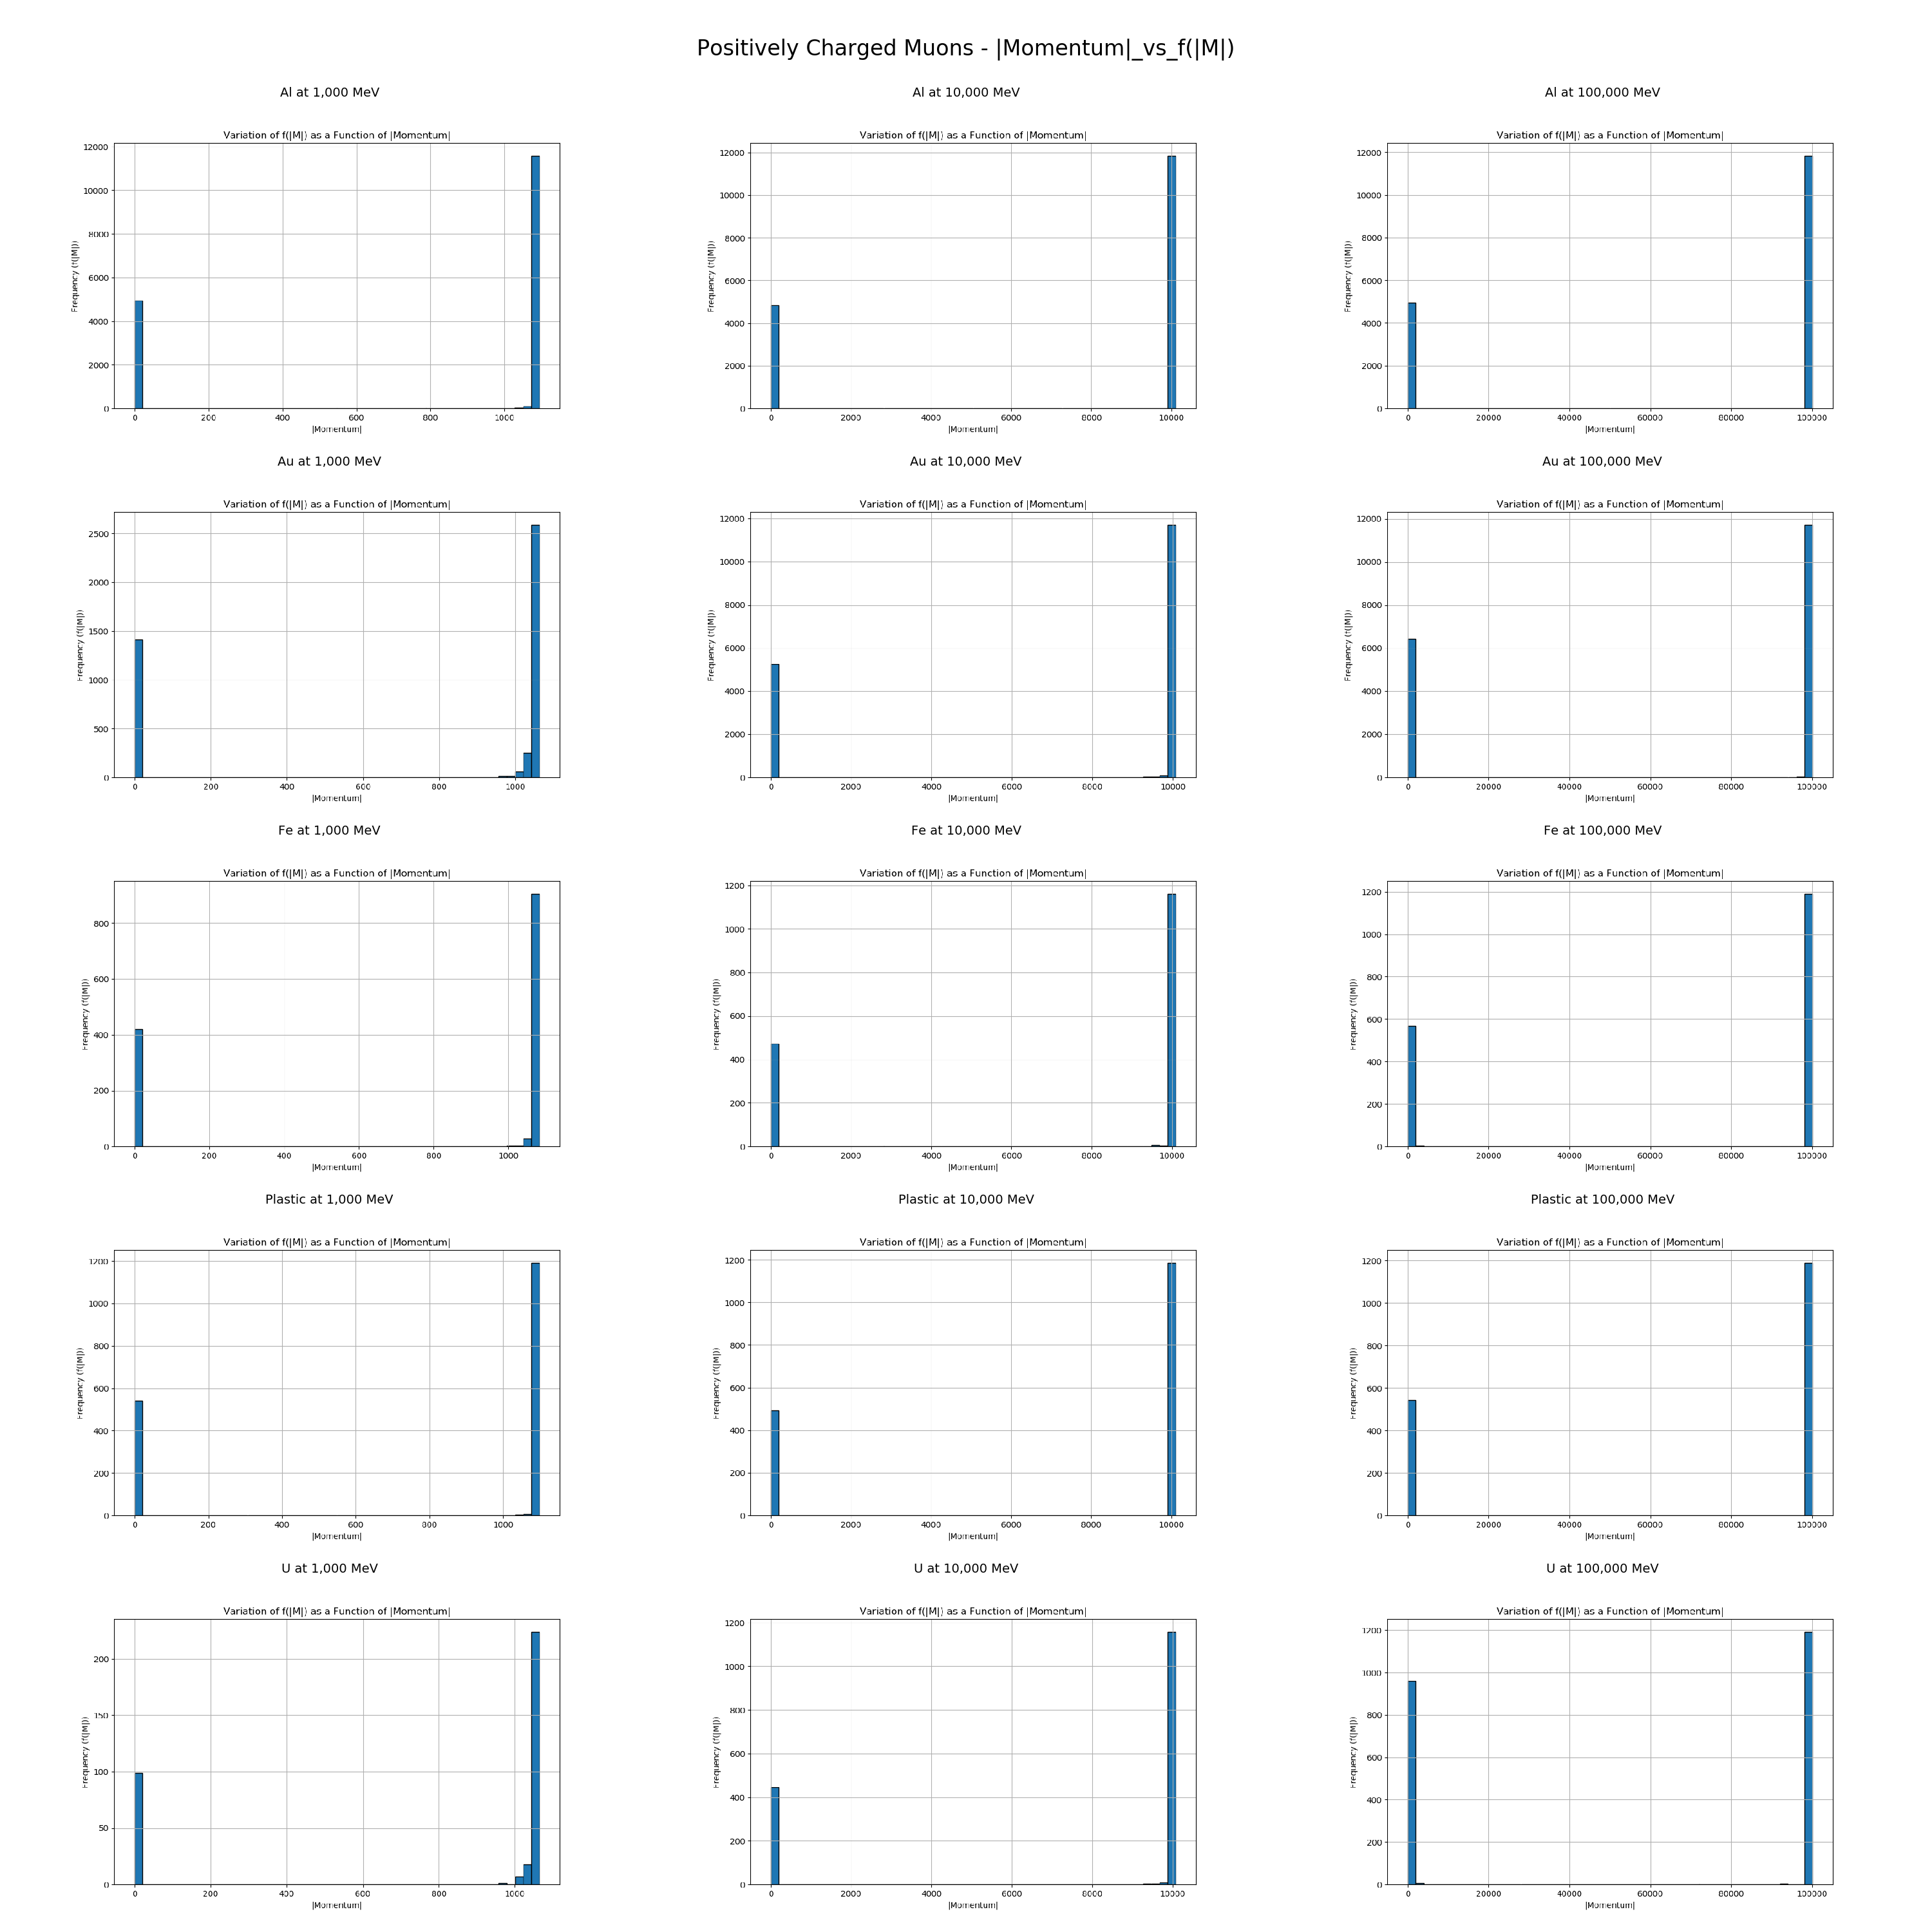
\includegraphics[width=0.9\textwidth]{images/Combined Plots/|Momentum|_vs_f(|M|)_mu+.png}
\end{figure}\

\noindent The histograms depicting the interactions of positively charged muons show that muons predominantly retain their initial momentum. At 1,000 MeV, peak frequencies are approximately 1,200 for Aluminum, Gold, Iron, and Uranium, and 200 for Plastic. At 10,000 MeV, peak frequencies are around 1,200 for all materials. At 100,000 MeV, the peak frequencies remain near 1,200 for all materials. The slight variations in frequency spread suggest minimal momentum change during interactions, with metals showing sharper peaks compared to the broader distribution in Plastic. These results indicate that muons maintain their momentum across different materials and energy levels, highlighting their robustness for experimental and material science applications.

\subsubsection{Negatively Charged Muons}

\begin{figure}[H]
\centering
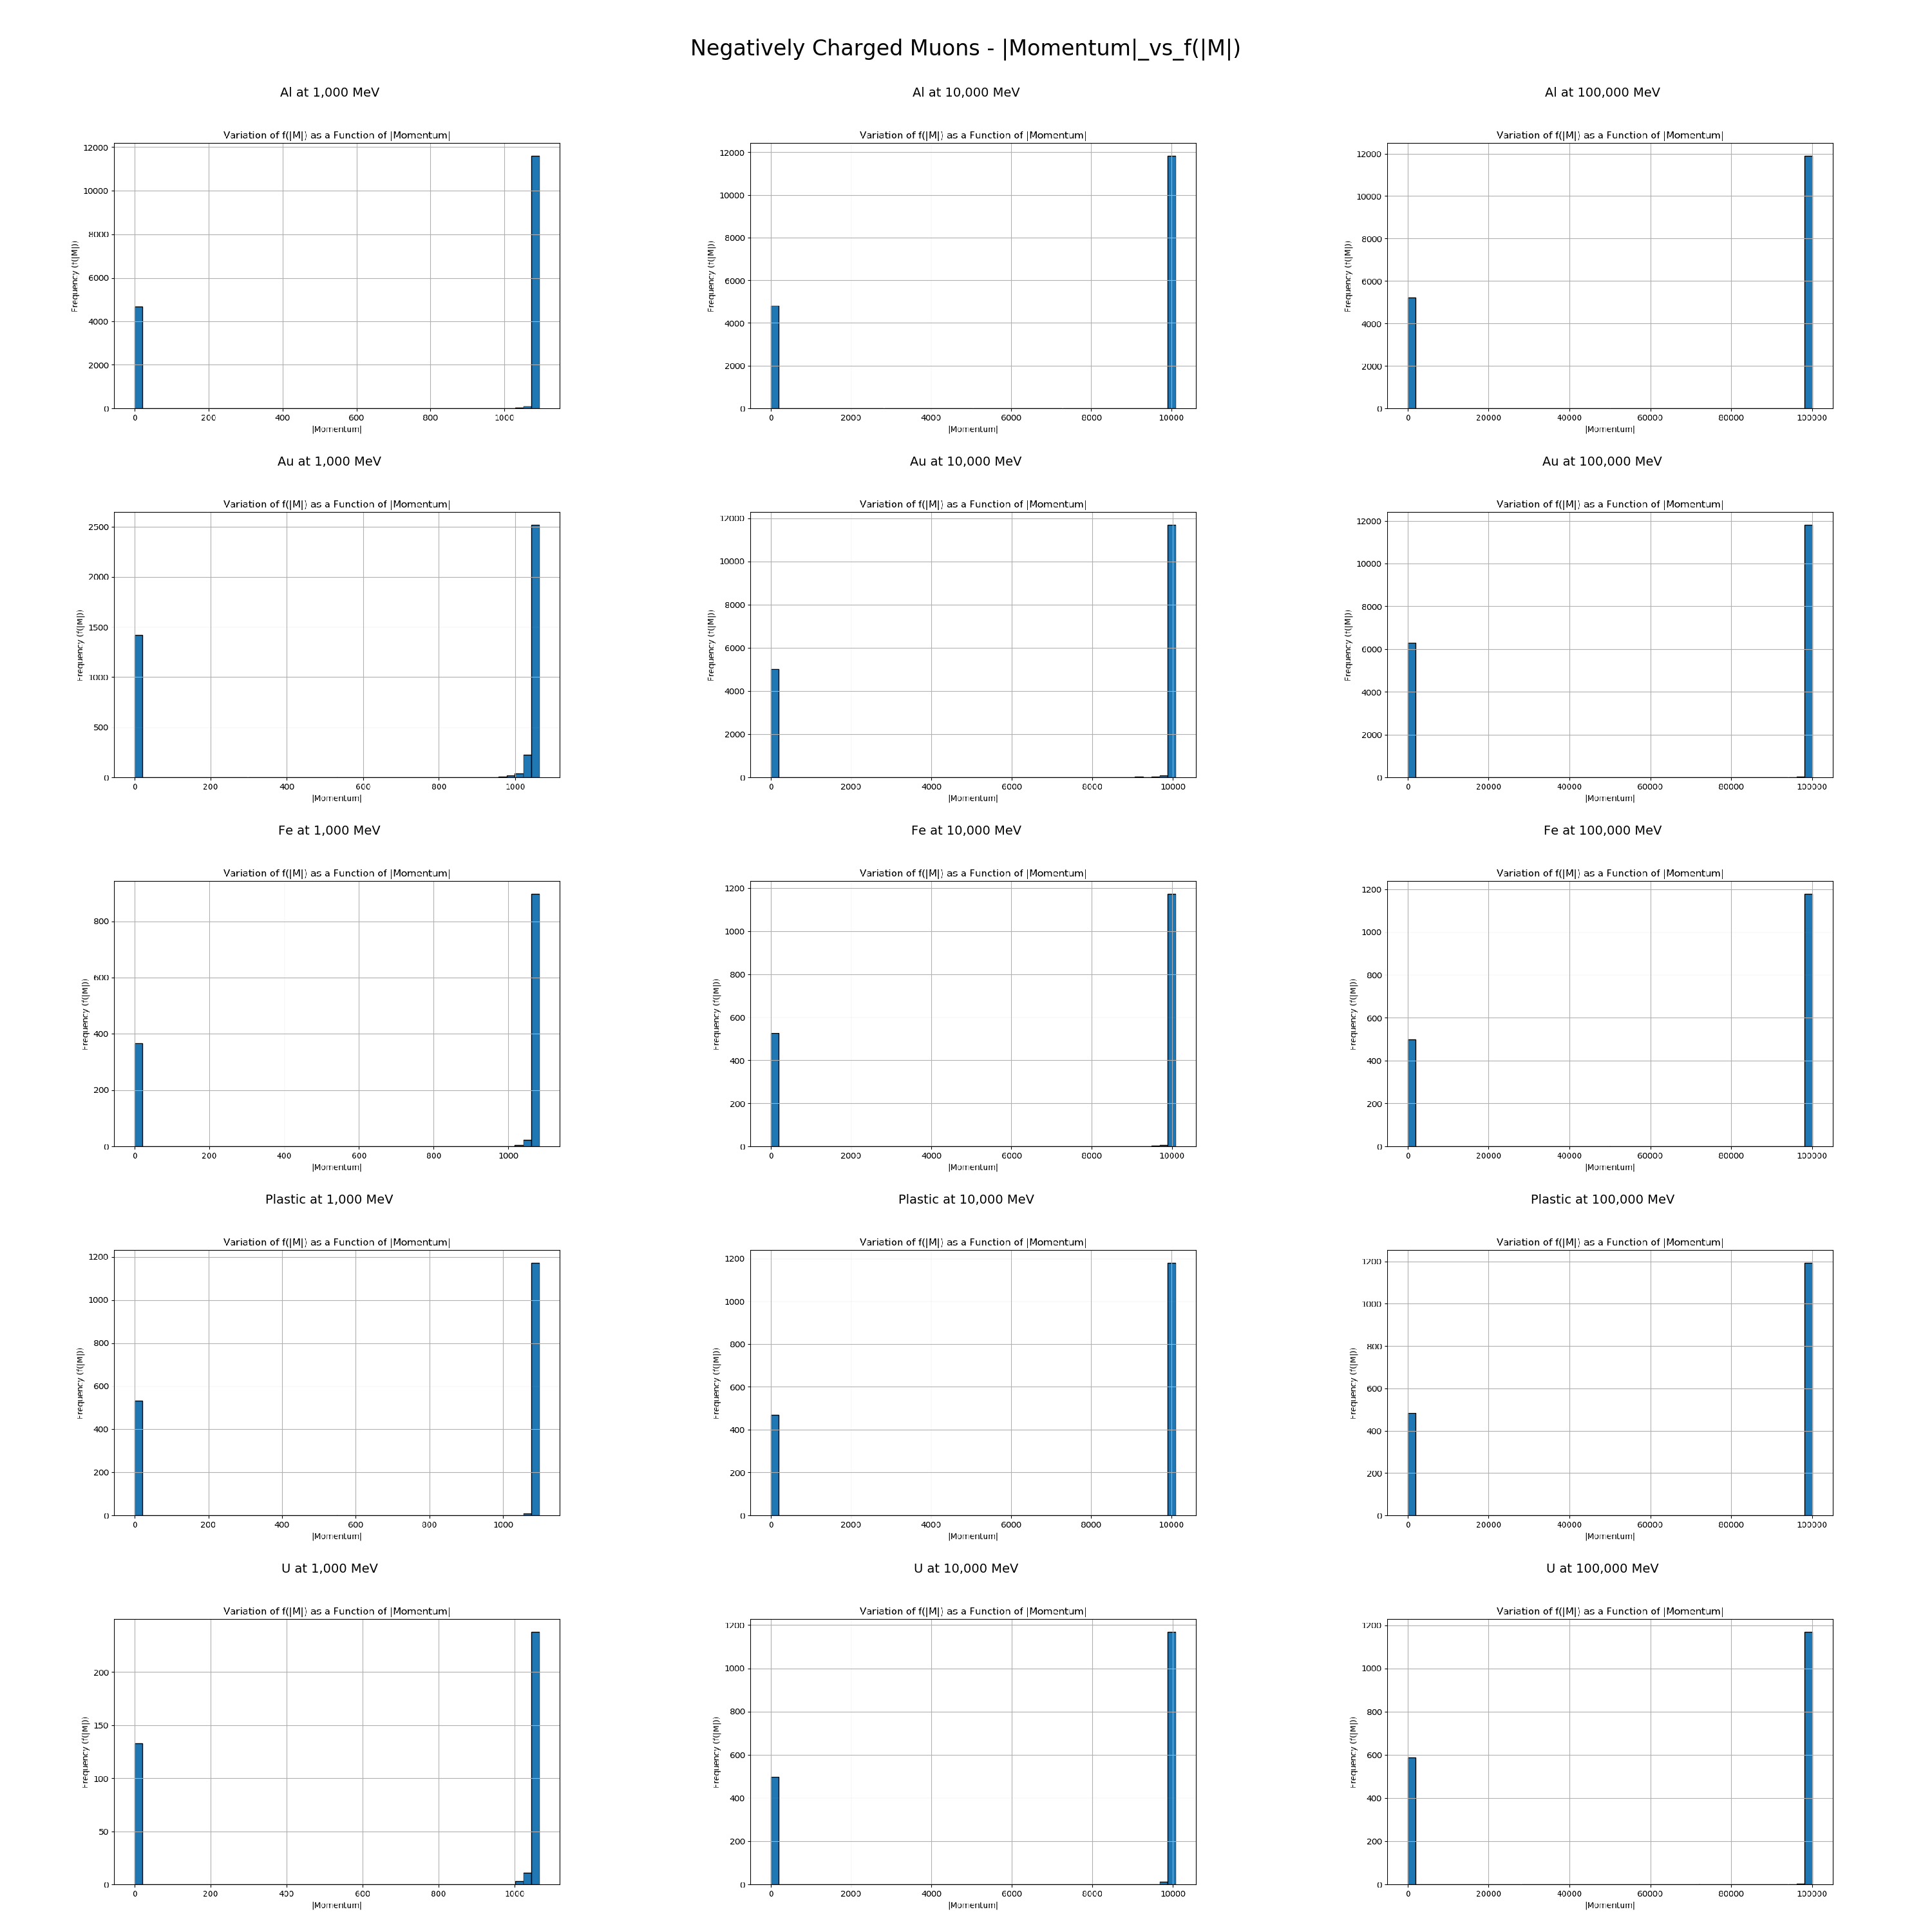
\includegraphics[width=0.9\textwidth]{images/Combined Plots/|Momentum|_vs_f(|M|)_mu-.png}
\end{figure}\

\noindent This histogram illustrates a consistent pattern in the momentum distribution of negatively charged muons. Each graph shows two distinct peaks: one at low momentum values (0-50 MeV/c) and another at high momentum values corresponding to the initial energy levels (1,000 MeV/c, 10,000 MeV/c, 100,000 MeV/c). For example, in the Aluminum graphs, the low momentum peak frequency is approximately 4,000-5,000 for 1,000 MeV, 6,000-7,000 for 10,000 MeV, and 6,000-7,000 for 100,000 MeV. In Gold, the low momentum peak frequency is around 1,200-1,300 across all energy levels. The high momentum peaks consistently show frequencies of 12,000-13,000, indicating muons that retain their initial energy. This pattern demonstrates the similar interaction mechanisms of muons with different materials, highlighting both rapid energy loss and energy retention behaviors.

\pagebreak

\section*{Acknowledgements}
I want to thank the Institute for Computing in Research for providing this opportunity and my mentor, Konstantin Borozdin for helping me out with my research at the institute in particle physics.

\bibliographystyle{johd}
\bibliography{bib}
\cite{YouTubePlaylist}
\cite{GitHubGeant4}
\cite{PDG2024}
\cite{MITOCW2020}

\end{document}